\documentclass[a4paper,11pt]{article}

\usepackage[english]{babel}
\usepackage[utf8x]{inputenc}
\usepackage{amsmath}
\usepackage{graphicx}
\usepackage{amsmath}
\usepackage{graphicx}
\usepackage[margin=0.5in]{geometry}
\usepackage{caption}
\usepackage{subfig}
\usepackage{epstopdf}
\usepackage{amssymb}

\title{Convergent Cross-Mapping and Causality Detection}
\author{McCracken,Weigel}

\begin{document}
\maketitle

\abstract{
Convergent Cross-Mapping is a technique, introduced by Sugihara {\em et al.\ }\cite{Sugihara2012}, reported to be ``a necessary condition for causation'' capable of distinguishing causality from correlation in sets of time series data.  We will show that CCM correlations do not in general agree with intuitive concepts of ``driving'' and ``response'', and as such, relationships among CCM correlations should not be considered indicative of causality.  It is shown that the calculation of CCM correlations can, however, be modified to identify asymmetric relationships between pairs of time series data.  We introduce ``pairwise asymmetric inference'' (PAI) and present examples of its use in inferring relationships within complex systems.  The sensitivity of CCM correlations (and consequently, PAI) on embedding dimensions and lag times will be discussed.
}

\section{Introduction}
Modern time series analysis includes a handful of techniques meant to discern "driving" or "cause and effect" relationships between different data sets.  These techniques have found application in a wide range of fields including neuroscience (e.g.\ \cite{Kaminski2001}), economics (e.g.\ \cite{dufour1998,dufour2006}), climatology (e.g.\ \cite{mosedale2006}), and others.  General casual relationships in time series data are also being studied in an effort to understand causality itself (e.g.\ \cite{eichler2012}).  

To date, most techniques for ``causal inference'' in time series data fall into two broad categories, those related to transfer entropy and those related to Granger causality.  Transfer entropy (introduced in \cite{Schreiber2000}) and Granger causality (introduced in \cite{granger1969}) are known to be equivalent under certain conditions \cite{Barnett2009}.  In this article, we investigate a casual inference technique, called Convergent cross-mapping (CCM), that was recently introduced by Sugihara {\em et al.\ } in \cite{Sugihara2012}.  Currently, there is no evidence that CCM is related to either transfer entropy or Granger causality.

We will begin with a review of the work of Sugihara {\em et al.}, including working through the coupled logistic map example presented in \cite{Sugihara2012}.  We will then illustrate the dependence of CCM correlations on the embedding dimension and lag time parameters of the CCM algorithm.  Finally, we will introduce ``pairwise asymmetric inference'' (PAI) and use it to show that, even though CCM causality may not be physical causality, it can still be a useful tool in the analysis of complex time series data.

\section{Convergent Cross-Mapping}
CCM is described as a technique used to identify ``causality'' between time series and is intended to be useful in situations where Granger causality is known to be invalid (i.e.\ in dynamic systems that are ``nonseperable'' \cite{Sugihara2012}).  The authors state that CCM is a ``necessary condition for causation''.  It is well known \cite{Granger1980,liu2012,Roberts1985} that Granger causality is not causality as it is typically understood in physics.  It will be shown that a similar conclusion can be drawn regarding CCM causality. 

CCM is closely related to simplex projection \cite{Sugihara1990,Sugihara1990a}, which predicts a point in the times series $X$ at a time $t+1$, i.e.\ $X_{t+1}$, by using the points with the most similar histories to $X_t$.  Similarly, CCM uses points with the most similar histories to $X_t$ to estimate $Y_t$.  The CCM correlation is the squared correlation coefficient\footnote{This definition differs slightly from the original definition in \cite{Sugihara2012}, which just uses Pearson’s correlation coefficient.  We use the square of this value to avoid dealing with negative correlation values.  This subtle change in the definition does not affect the conclusions drawn in \cite{Sugihara2012}, as can be seen in our reproduction of key plots from that work.} between the original time series $Y$ and estimate of $Y$ made using the convergent cross-mapping with $X$, which is labeled as $Y|X$; i.e.\ the CCM correlation is given as 
$$
C_{YX} = \left(\rho\left(Y,Y|X\right)\right)^2\;\;,
$$
where $\rho(A,B)$ is the Pearson correlation coefficient between $A$ and $B$ \cite{}.  Any pair of times series, $X$ and $Y$, will have two CCM correlations, $C_{YX}$ and $C_{XY}$, which are compared to determine the CCM causality.  For example, Sugihara {\em et al.\ }define a difference of CCM correlations
\begin{equation}
\label{eqn:delta}
\Delta = C_{YX} - C_{XY}
\end{equation}
and use the sign of $\Delta$ to determine the CCM causality between $X$ and $Y$ \cite{Sugihara2012}.  The CCM algorithm is explained in more detail in Appendix \ref{sec:appA}.

If $X$ can be estimated from the shadow manifold of $Y$ better than $Y$ can be estimated from the shadow manifold of $X$ (e.g.\ if $\Delta < 0$), then $X$ is said to ``CCM cause'' $Y$.

\subsection{Simplified Two Population Dynamics}
\label{sec:2Pop}
Consider the example system used by Sugihara {\em et al.\ }in \cite{Sugihara2012}:
\begin{eqnarray}
\label{eqn:2pop}
X_t &=& X_{t-1}\left(r_x-r_x X_{t-1}-\beta_{xy} Y_{t-1}\right)\\
Y_t &=& Y_{t-1}\left(r_y-r_y Y_{t-1}-\beta_{yx} X_{t-1}\right)
\end{eqnarray}
where $r_x,r_y,\beta_{xy},\beta_{yx}\in\mathbf{R}\ge 0$.  This pair of equations is a specific form of the two-dimensional coupled logistic map system, which is known to be chaotic \cite{Lloyd1995}.

In this example, the CCM causality of this system is determined by sampling both the initial conditions and the dynamics parameters, calculating $\Delta$, and demonstrating the necessary convergence.  The dynamic parameters $r_x$ and $r_y$ are sampled from a normal distributions $N\left(\mu_{rx},\sigma_{rx}\right)$ and $N\left(\mu_{ry},\sigma_{ry}\right)$, respectively.  The initial conditions $X_0$ and $Y_0$ are also sampled for normal distributions, specifically $N\left(\mu_{x0},\sigma_{x0}\right)$ and $N\left(\mu_{y0},\sigma_{y0}\right)$.  The coupling parameters $\beta_{xy}$ and $\beta_{yx}$ are then varied over the interval $[10^{-6},1]$ (in steps of {\bf ????}) to produce the plots seen in Figure \ref{fig:}.

Sugihara {\em et al.\ }consider convergence to be critically important to determining CCM causality, identifying it as ``a key property that distinguishes causation from simple correlation'' \cite{Sugihara2012}.  Figure \ref{fig:} shows plots created with several different library lengths to illustrate the convergence of $\Delta$ for this example.  Typically, for convenience, the (approximately) converged CCM correlation values will be reported and proof of convergence will be implied, rather than shown.
\begin{figure}[ht]
\label{fig:}
\begin{tabular}{cc}
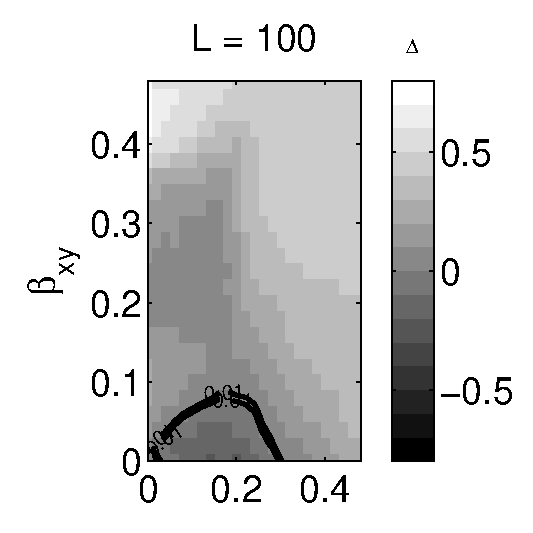
\includegraphics[scale=0.9]{Figure1A.eps} & 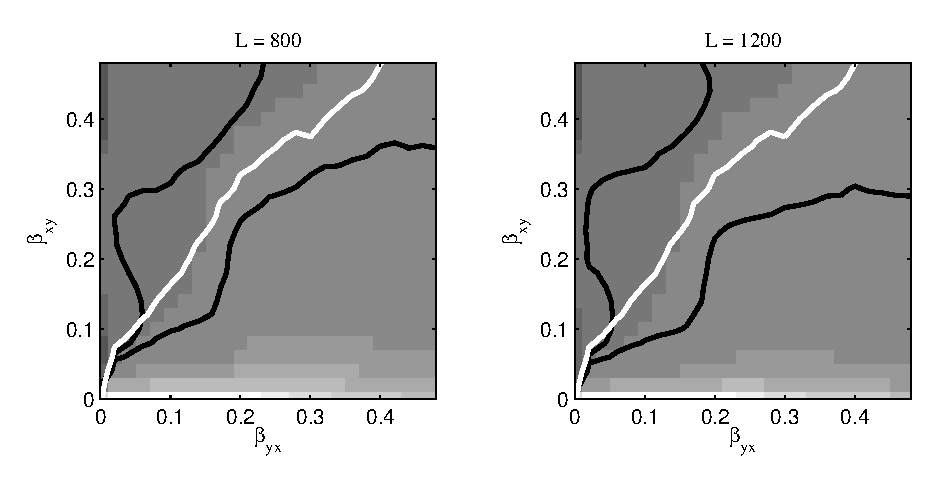
\includegraphics[scale=0.9]{Figure1B.eps}\\
(a) & (b) \\[6pt]
%\includegraphics[scale=0.6]{Figure1C.eps} & \includegraphics[scale=0.6]{Figure1D.eps}\\
 & \\
(c) & (d) \\[6pt]
\end{tabular}
\caption{These plots show the dependence of Eqn.\ \ref{eqn:delta} on $\beta_{xy}$ and $\beta_{yx}$.  See the text for details on how these plots were created along with a discussion of the interpretation of these plots in terms of the CCM causality.}
\end{figure}
\begin{figure}[ht]
\label{fig:}
\begin{tabular}{cc}
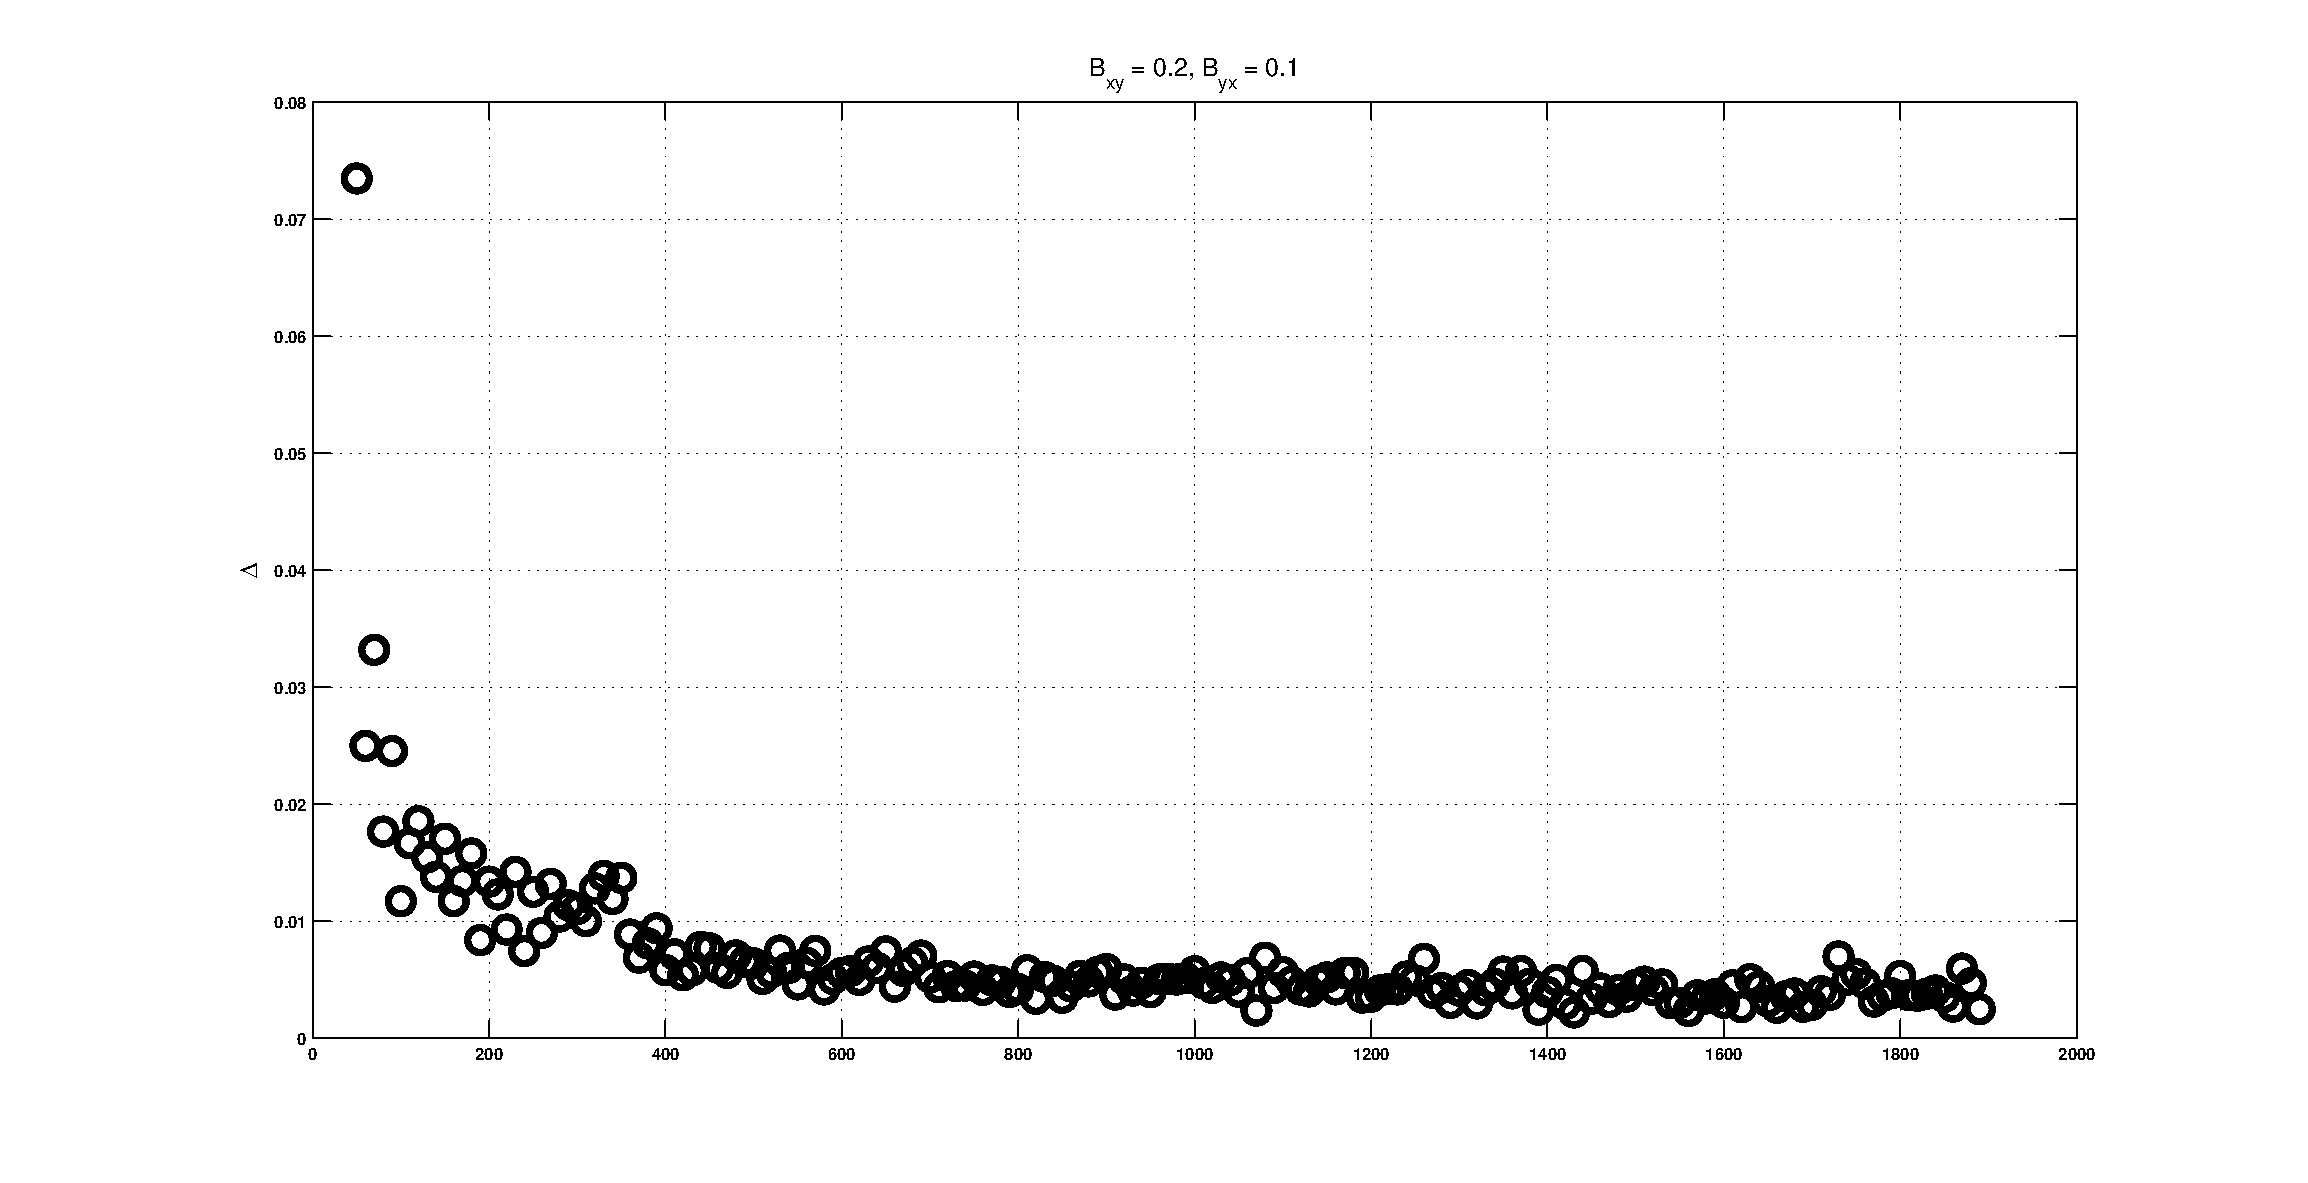
\includegraphics[scale=0.9]{RefFigureA.eps} & 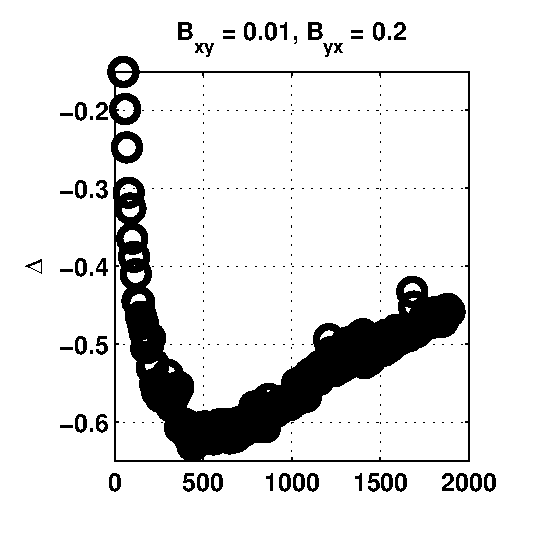
\includegraphics[scale=0.9]{RefFigureB.eps}\\
(a) $\beta_xy = ??,\;\beta_yx=?$ & (b) $\beta_xy = ??,\;\beta_yx=?$\\[6pt]
\end{tabular}
\caption{Reference figure.}
\end{figure}

The idea is that $\beta_{xy}>\beta_{yx}$ intuitively implies $Y$ ``drives'' $X$ more than $X$ ``drives'' $Y$.  Stated more formally, $\beta_{xy}>\beta_{yx}\Rightarrow\Delta>0$, which is reported as ``$Y$ CCM causes $X$''.  Likewise, $\beta_{xy}<\beta_{yx}$ implies $X$ CCM causes $Y$ and $\beta_{xy}=\beta_{yx}$ implies no CCM causality in the system.  It will be shown below that CCM causality is not necessarily related to causality as it is typically understood in physics.

\section{Embedding Dimension and Lag Time}
The CCM algorithm depends on the embedding dimension $E$ and the lag time step $\tau$ (see Appendix \ref{sec:appA}).  Consider the simplified two population system (Eqn.\ \ref{eqn:2pop}) with $r_x=3.8$, $r_y=3.5$, $\beta_{xy}=0.01$, $\beta_{yx}=0.2$, $X_0=0.4$, and $Y_0=0.2$ with $X$ and $Y$ library lengths of $L=2000$.  Figure \ref{fig:Etau} shows the effect of varying $E$ and $\tau$ on $\Delta$ for this system.  $E$ is varied over the interval $[2,20]$ (in steps of 1), and $\tau$ is varied over the interval $[1,50]$ (also in steps of 1).  This figure makes it clear that a statement of CCM causality (and, subsequently, that statement's agreement with intuition) depends strongly upon how the CCM technique is used.
\begin{figure}[ht]
\label{fig:Etau}
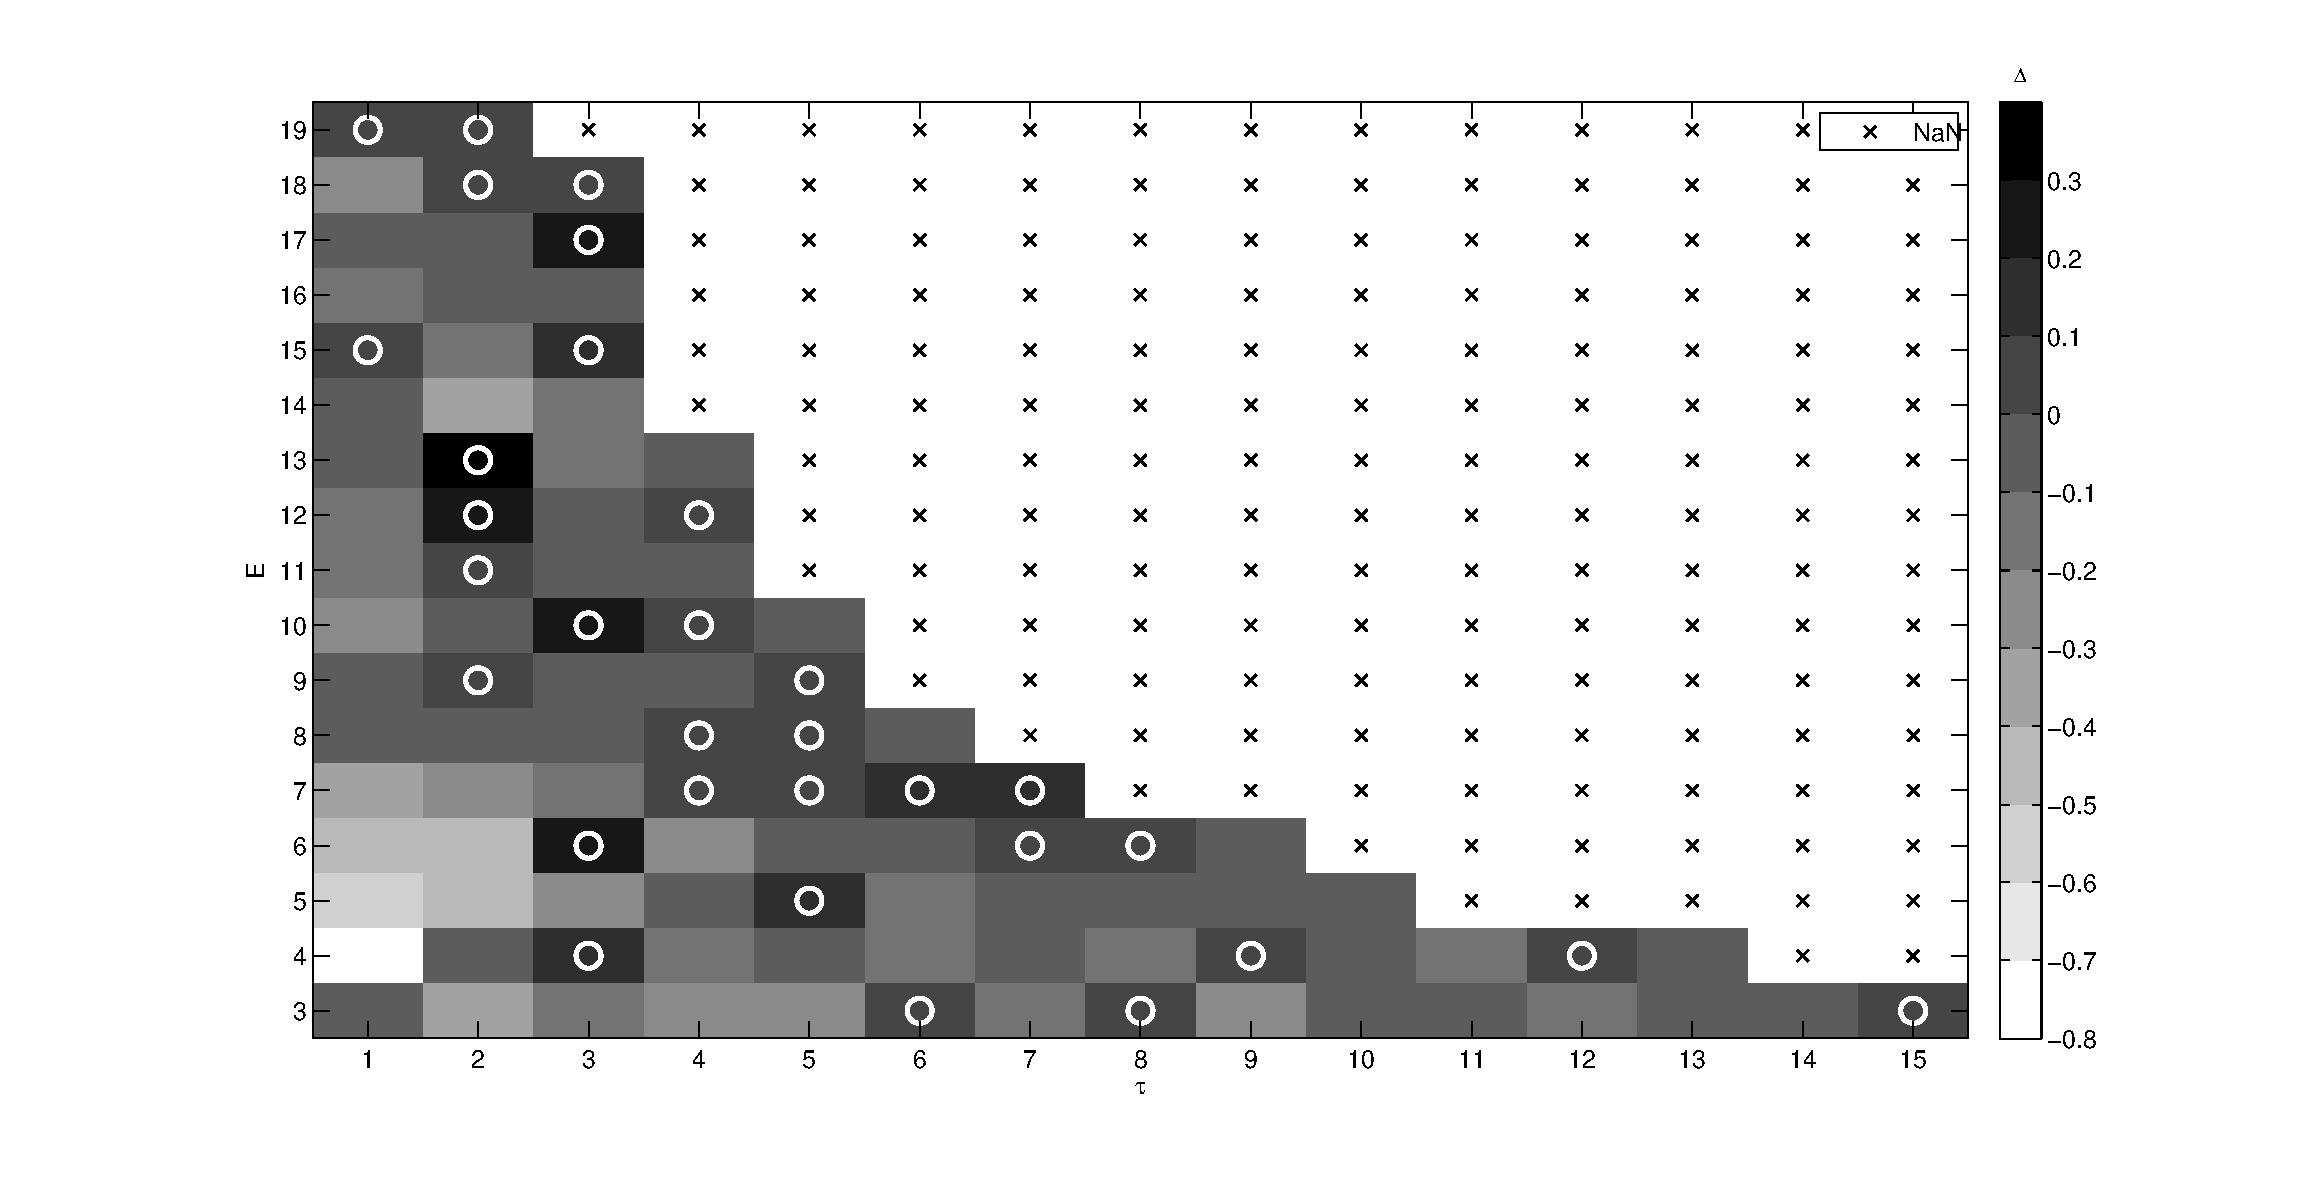
\includegraphics[scale=0.45]{Figure2.eps}\\
\caption{The determination of CCM causality in a system is dependent on the CCM parameters of embedding dimension $E$ and lag time step $\tau$.  This plot show the dependence of Eqn.\ \ref{eqn:delta} on $E$ and $\tau$ for the example system discussed in the text.}
\end{figure}
A dependence $E$ and $\tau$ is a feature of most state space reconstruction (SSR) methods \cite{Hong2006,vlachos2009,Small2004}.  CCM is related to state space reconstruction \cite{Sugihara2012}, so the $E$ and $\tau$ dependence seen here is not unexpected.  Sugihara {\em et al.\ }do not discuss in depth how to determine $E$ and $\tau$, but they do mention that ``optimal embedding dimensions'' are found using univariate SSR \cite{Sugihara2012} (supplementary material).  Other methods for determining $E$ and $\tau$ for SSR algorithms can be found in the literature (e.g. cite ???).

\section{Simple Example Systems}
The usefulness of the CCM algorithm in identifying causal or driving structure among sets of time series can be explored by using simple example systems.  Each of the following examples intuitively supports the conclusion that $X$ drives $Y$, and applying the CCM algorithm (with $E=3$ and $\tau=1$) leads to conclusions that do not always agree with this intuition.

\subsection{Linear Example}
Consider the linear example dynamical system of
\begin{eqnarray}
\label{eq:linearex}
X_t &=& \sin(t)\\
Y_t &=& AX_{t-1}+B\eta_t,
\end{eqnarray}
with $A,B\in\mathbb{R}\ge 0$ and $\eta_t\sim\mathcal{N}\left(0,1\right)$.  Specifically, consider $A,B\in[0,10]$ in increments of 0.1.  Figure \ref{fig:linearex1} shows $\Delta$ for this example given a library length of $L=2000$.
\begin{center}
\begin{figure}[ht]
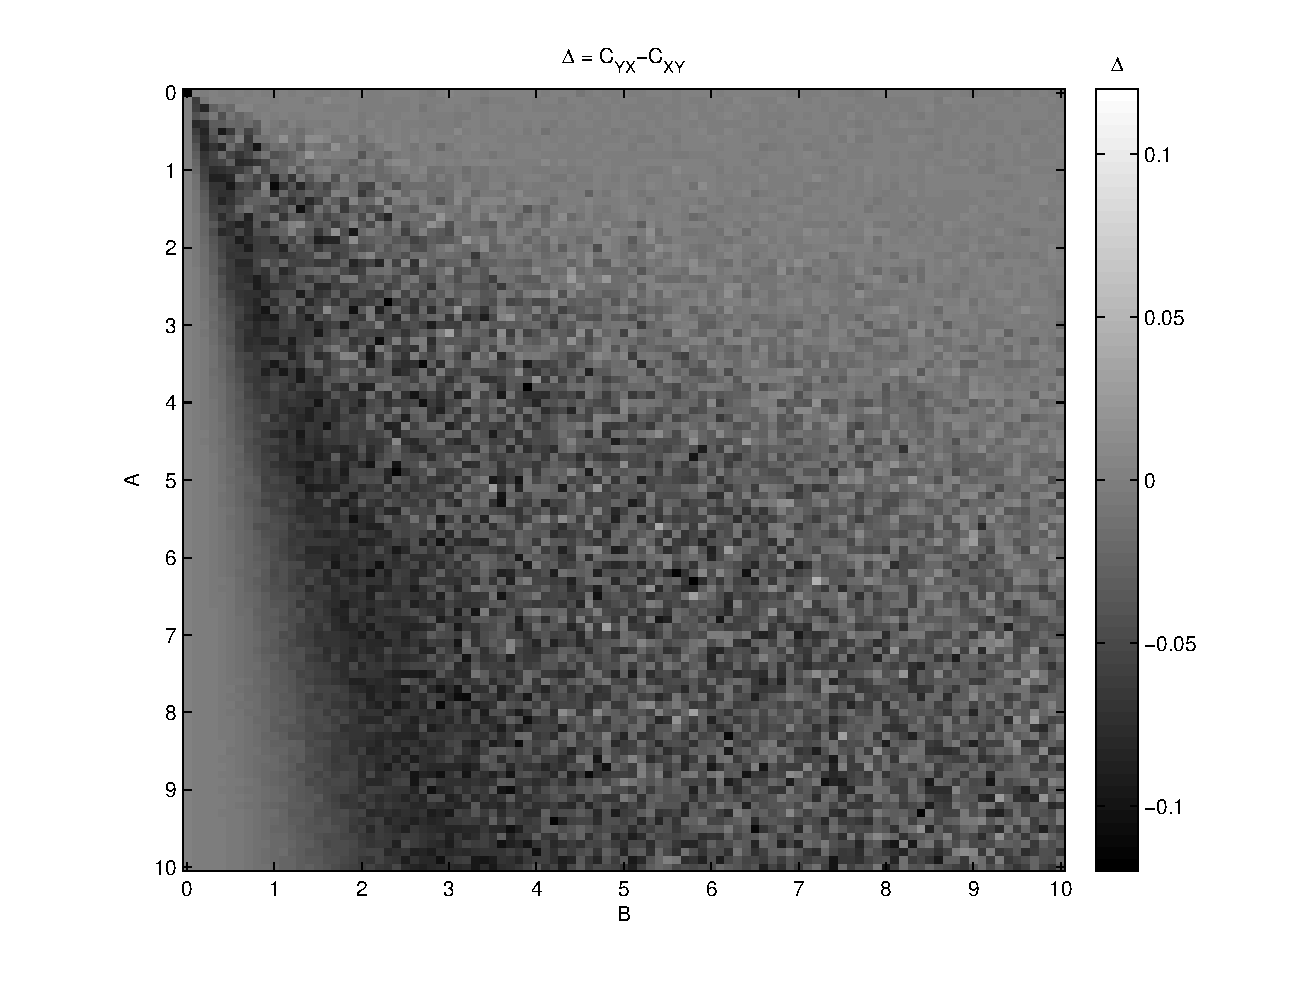
\includegraphics[scale=0.7]{RLCircuitPlots/LinearEx_Delta.eps} \\
\caption{Changing $A$ and $B$. $\Delta$}
\label{fig:linearex1}
\end{figure}
\end{center}
\begin{center}
\begin{figure}[ht]
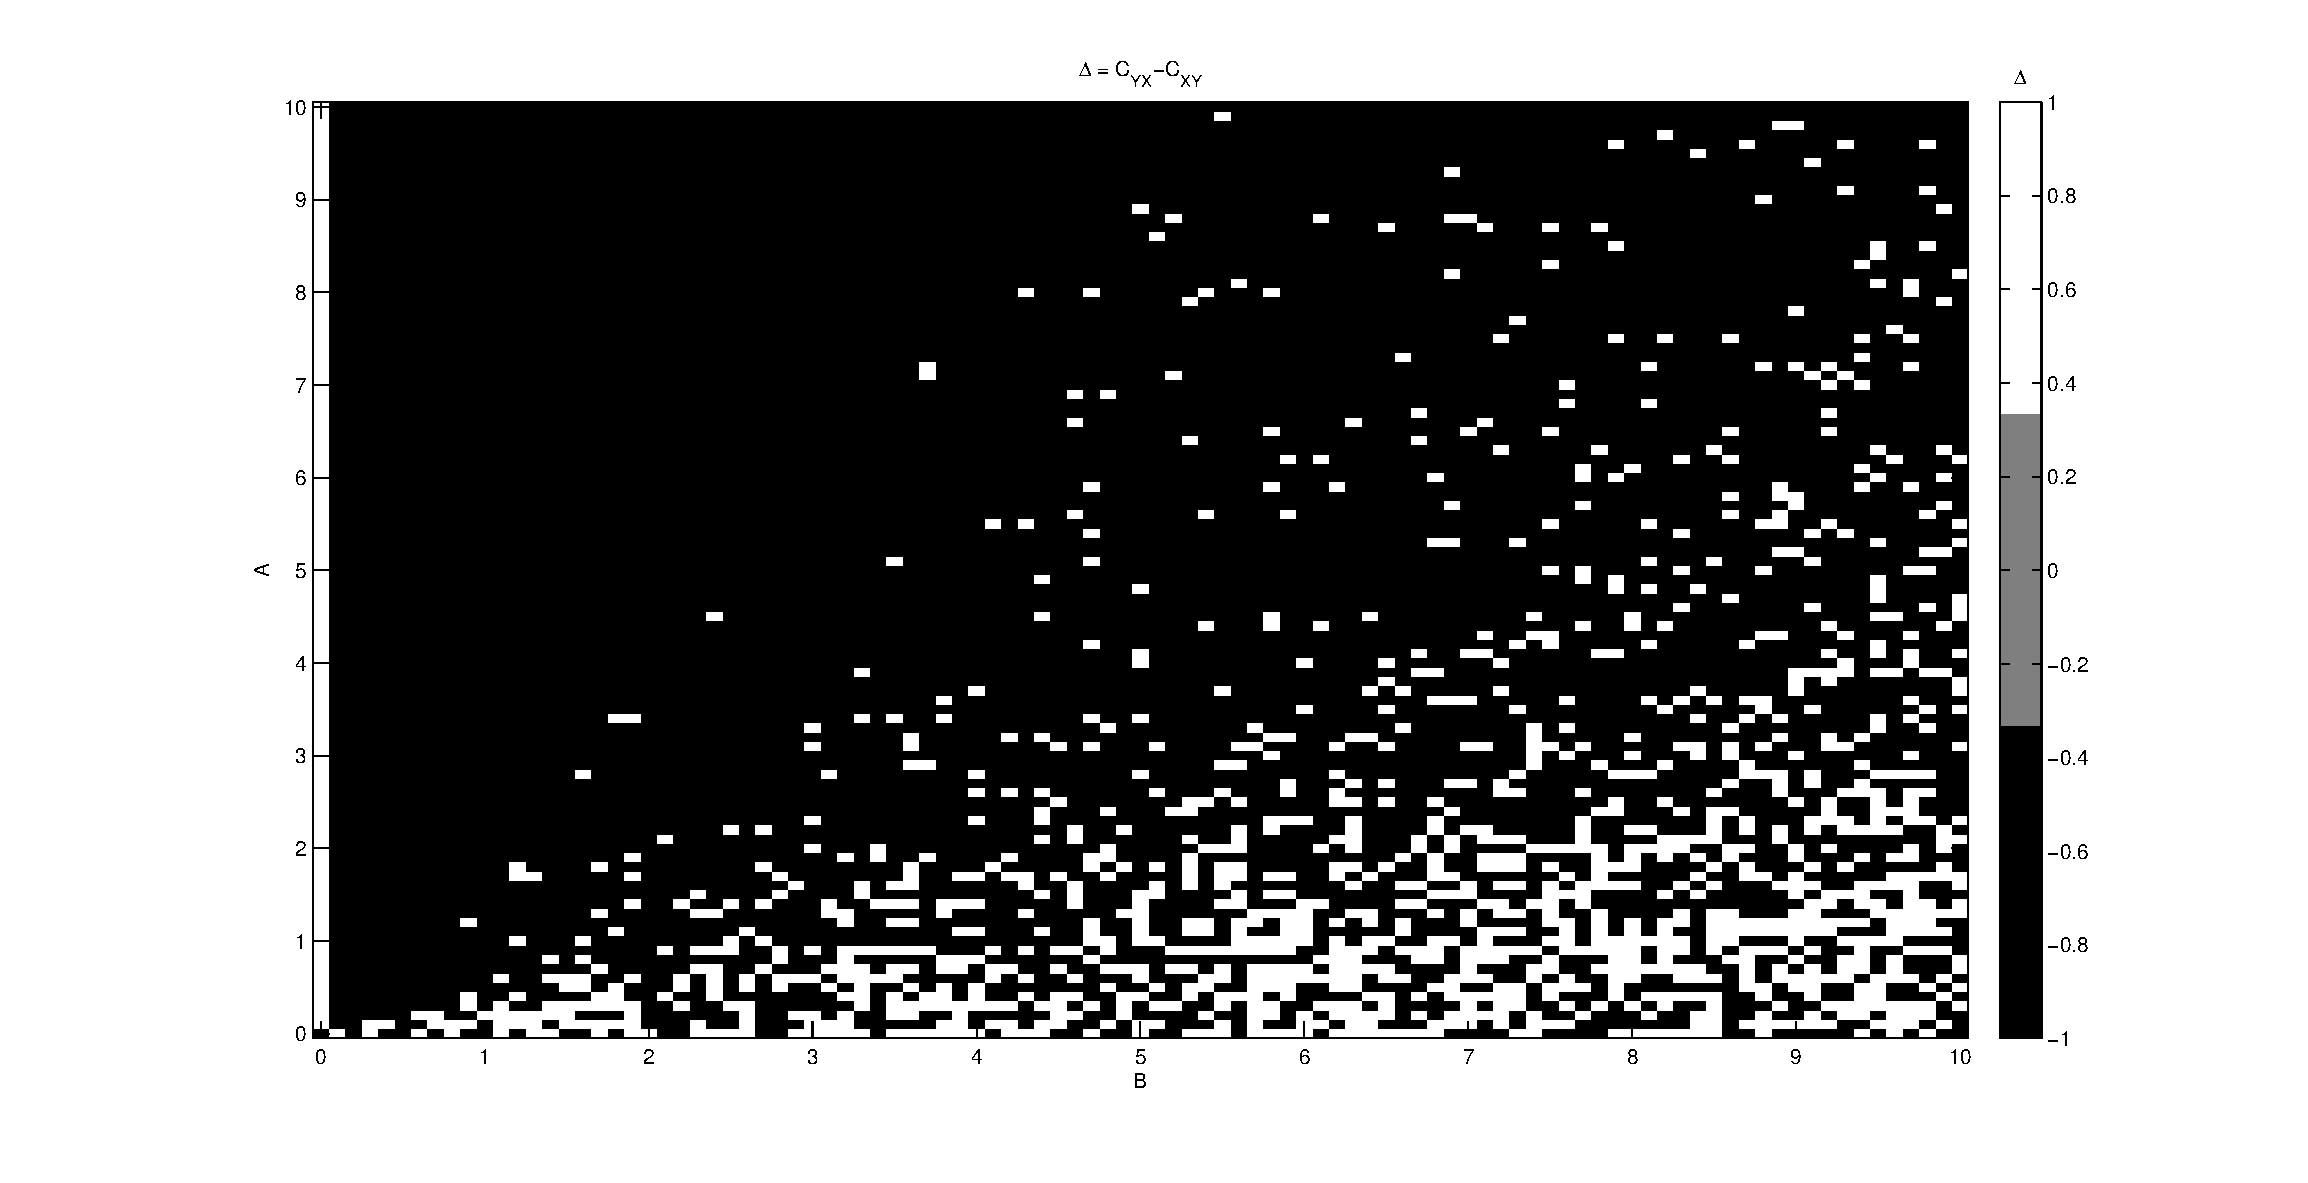
\includegraphics[scale=0.55]{LinearEx3colortemp.eps} \\
\caption{Changing $A$ and $B$. $\Delta$}
\label{fig:linearex1}
\end{figure}
\end{center}
The convergence of two specific points in Figure \ref{fig:linearex1}, $(A,B) = (2.6,2.6)$ and $(A,B)=(3.0,2.6)$, is shown in Figure \ref{fig:linearex1a}.
\begin{center}
\begin{figure}[ht]
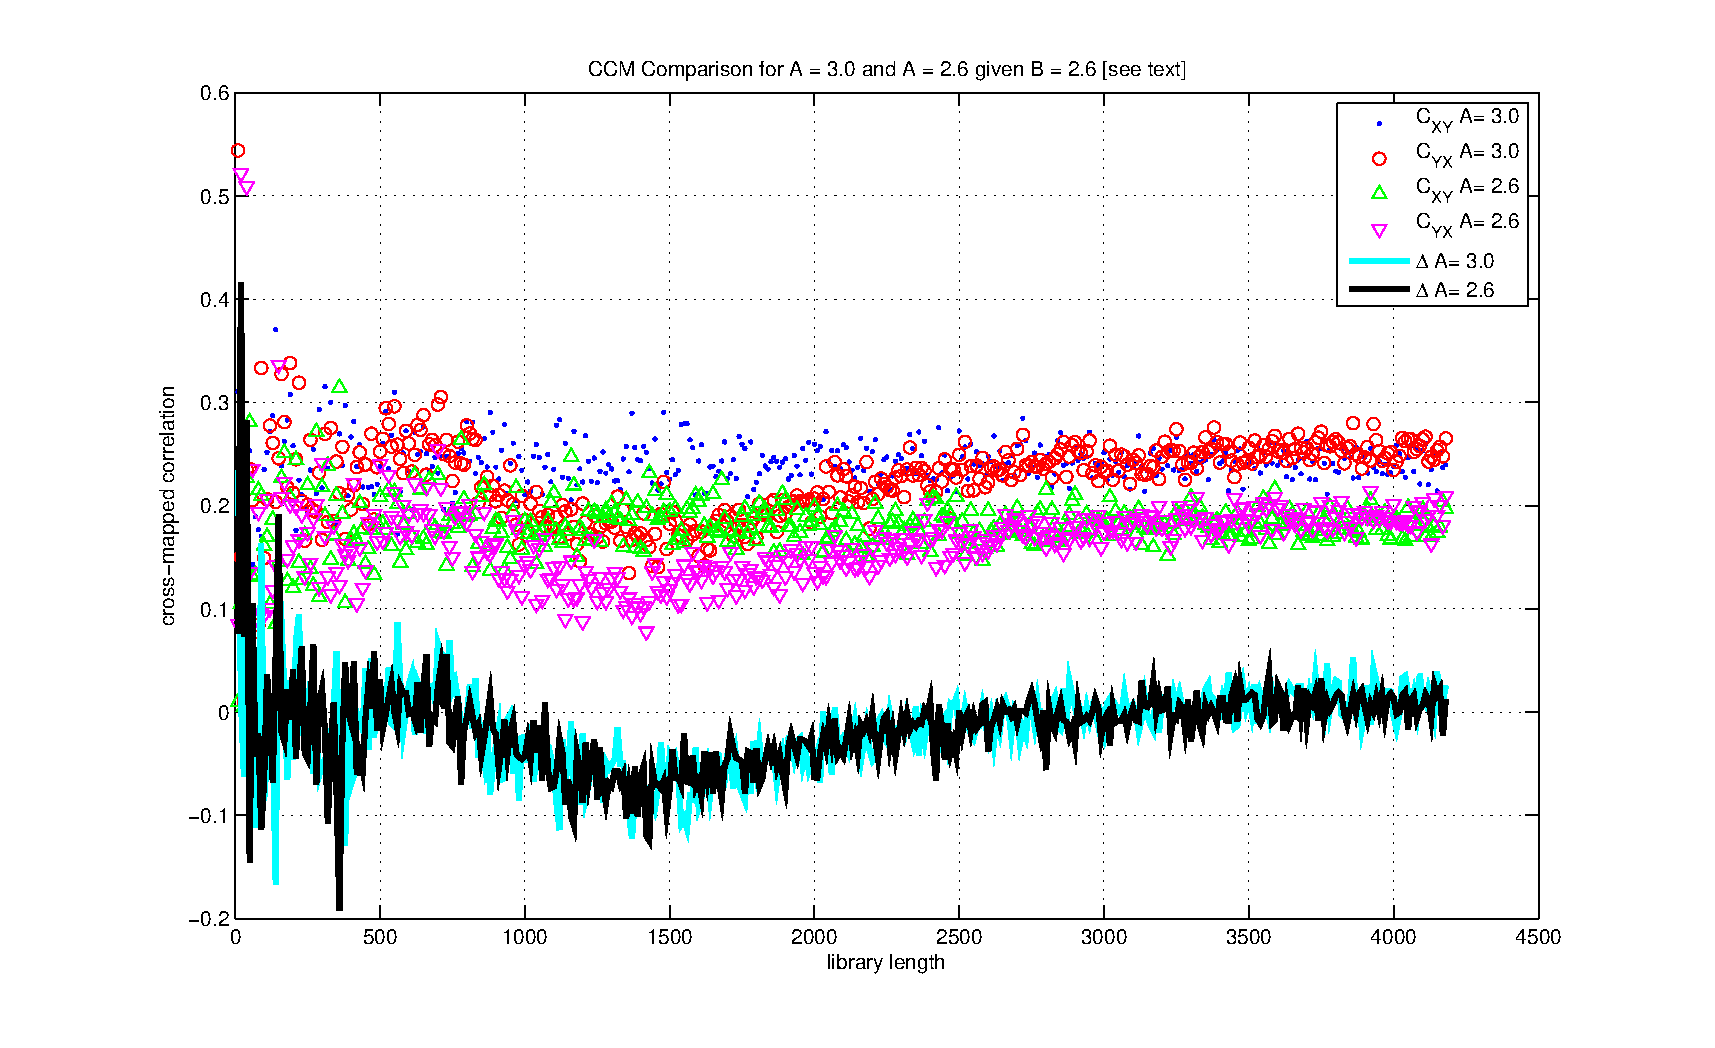
\includegraphics[scale=0.7]{RLCircuitPlots/LinearEx_ChangeL.eps} \\
\caption{}
\label{fig:linearex1a}
\end{figure}
\end{center}
The expected conclusion of $X$ drives $Y$ would correspond to  $X$ CCM causes $Y$, which implies $\Delta<0$.  But, it can be seen from the plots above that the sign of $\Delta$ changes as $A$ and $B$ change.  Given that the intuitive conclusion of $X$ drives $Y$ in Eqn.\ \ref{eq:linearex} does not depend on $A$ and $B$, it would seem that $\Delta$ does not reliably reflect the intuitive conclusion in this linear example system.  

Figure \ref{fig:linearex1a} shows (for the two specific points plotted) that $\Delta$ is more negative at shorter library length but appears to converge to a point near zero as the library length is increased.  The convergence of CCM correlations is emphasized \cite{Sugihara2012}, so the seemingly counter intuitive behavior of $\Delta$ (and $C_{XY}$ and $C_{YX}$) in Figure \ref{fig:linearex1a} again seems to imply that the CCM correlations may not be a reliable measure of ``driving'' (at least not the intuitive definition) for this simple linear example system.

\subsection{Non-Linear Example}
Consider the nonlinear example dynamical system of
\begin{eqnarray}
X_t &=& \sin(t)\\
Y_t &=& AX_{t-1}\left(1-BX_{t-1}\right)+C\eta_t,
\end{eqnarray}
with $A,B,C\in\mathbb{R}\ge 0$ and $\eta_t\sim\mathcal{N}\left(0,1\right)$.  Specifically, consider $A,B,C\in[0,5]$ in increments of 0.5.  Figure \ref{fig:nonlinearex} shows $\Delta$ for specific values of $C$ given a library length of $L=??$.
\begin{figure}[ht]
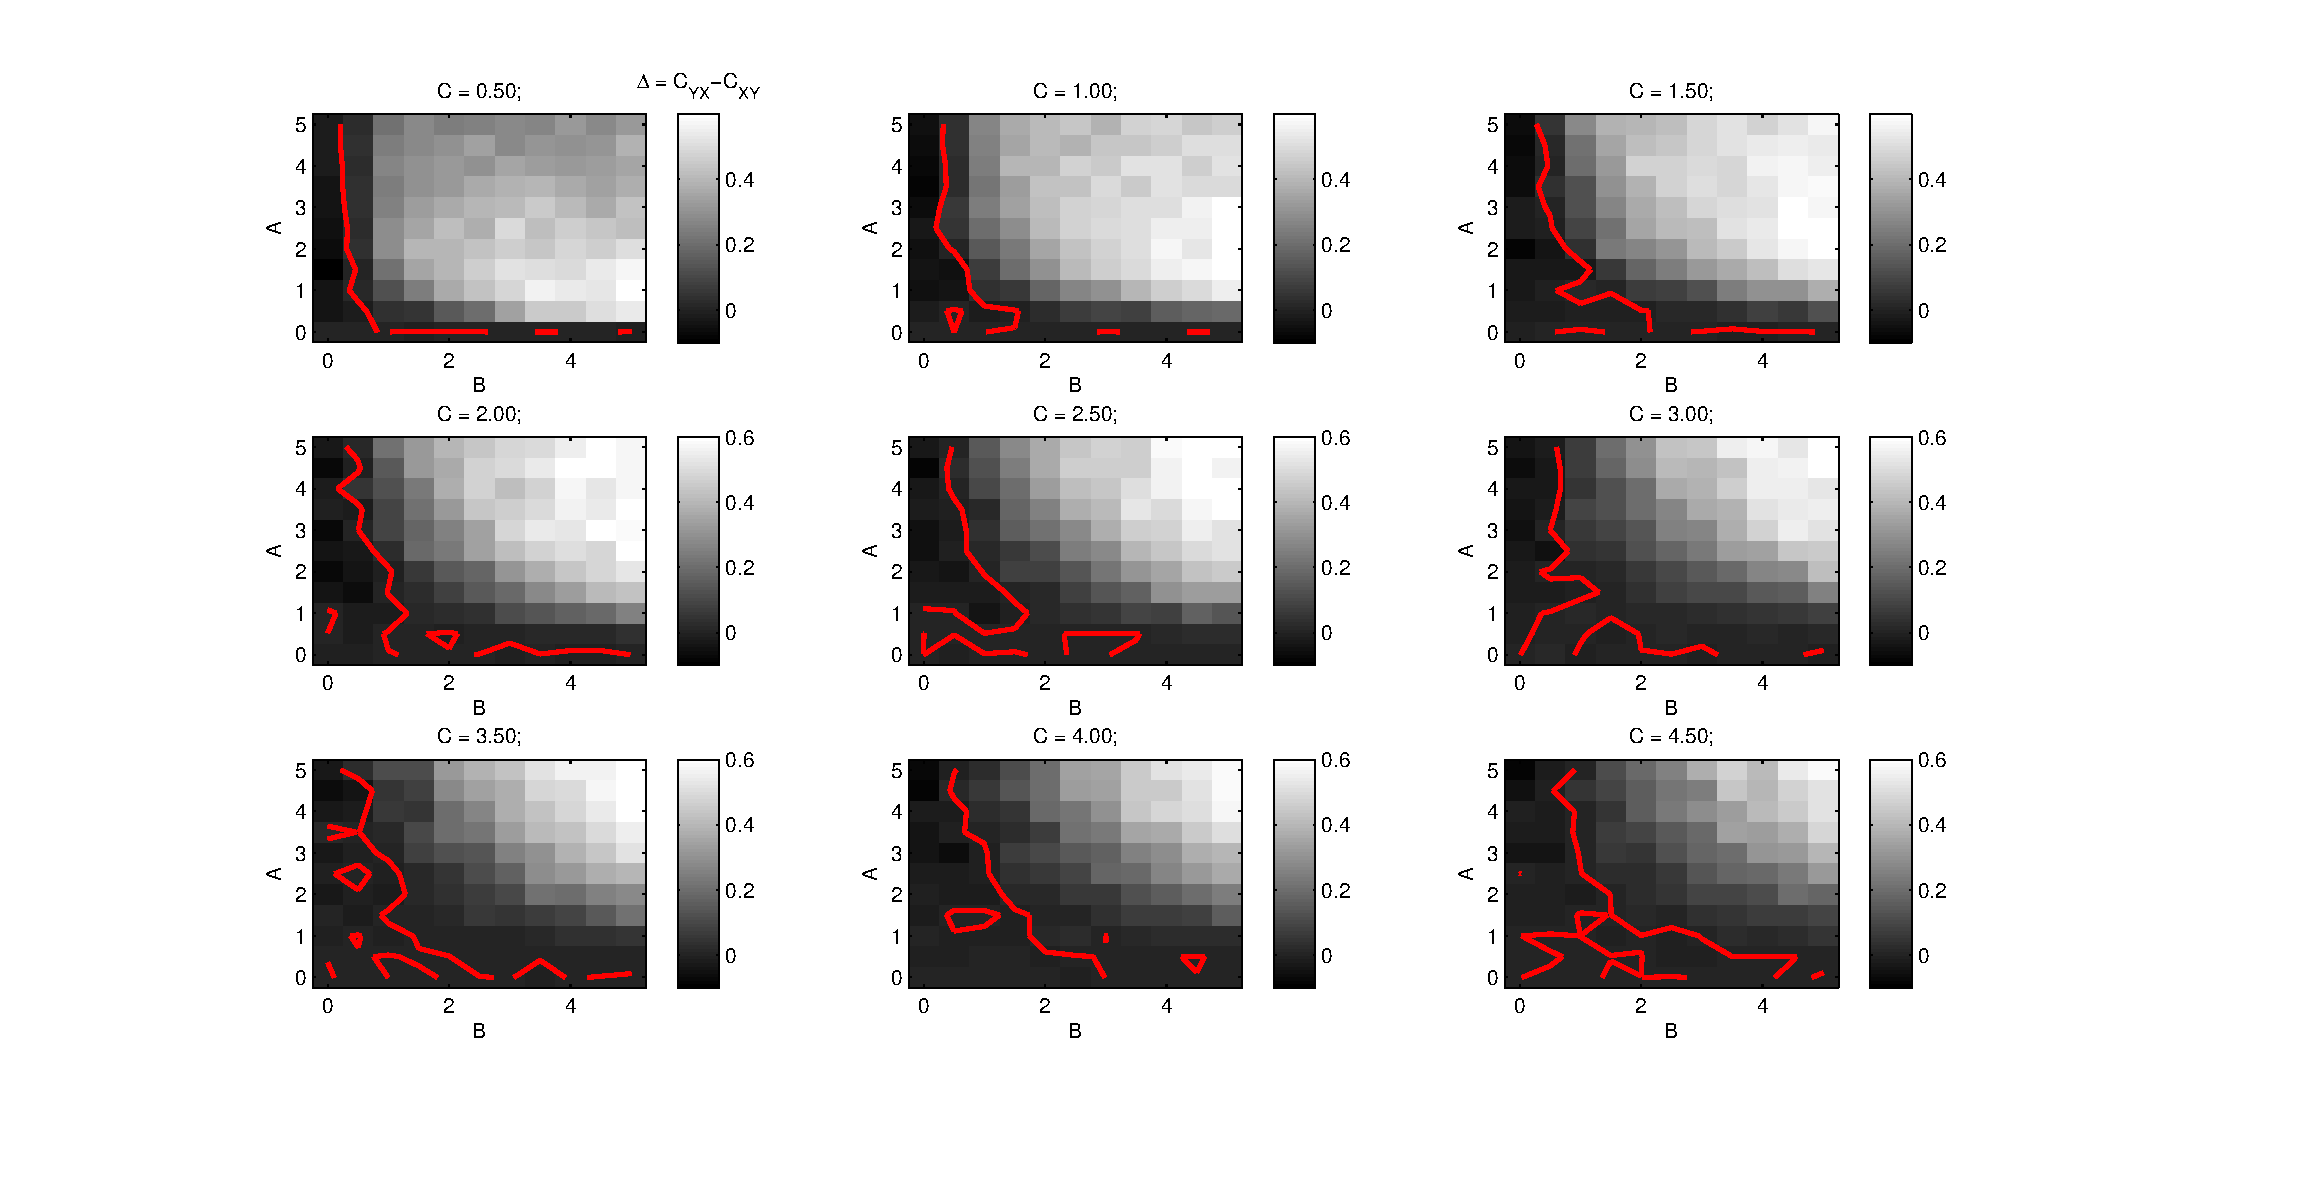
\includegraphics[scale=0.55]{RLCircuitPlots/NonLinearEx.eps} \\
\caption{}
\label{fig:nonlinearex}
\end{figure}
Just as in the previous linear example, the expectation for this example system is that $\Delta<0$ independent of the parameters $A$, $B$, and $C$.  However, it can be seen from the plots that the sign of $\Delta$ can depend on all three parameters.  Thus this simple non-linear example leads to a similar conclusion to the previous linear example; i.e. $\Delta$ does not appear to reliably reflect intuitive notions of driving.

\section{RL Circuit Example}
Both of the previous examples included a noise term, $\eta_t$ (which was not averaged over in any way).  The failure of CCM correlations to meet expectations in the previous examples may be considered a failure of the algorithm's ability to deal with noise.  This idea can be investigated by considered a system without stochastic noise terms.  To that end, consider the familiar physical system of a electrical circuit containing a resistor and an inductor.

The continuous system is
\begin{equation}
\label{eqn:it}
\frac{dI}{dt} = \frac{V(t)}{L} - \frac{R(t)}{L} I,
\end{equation}
where $I$ is the current at time $t$, $V(t)$ is the voltage at time $t$, $R(t)$ is the resistance at time $t$, and $L$ is the inductance (which is also constant in these examples), and it can be approximated as
\begin{equation}
\dot{I} = \frac{V(t)}{L} - \frac{R(t)}{L} I\Rightarrow I_{t+1}-I_t = \frac{V_t}{L} - \frac{R_t}{L} I_t.
\end{equation}
Rearranging leads to
\begin{eqnarray}
I_{t+1} &=& \frac{V_t}{L}+I_t\left(1-\frac{R_t}{L}\right),\\
V_t &=& L\left(I_{t+1}-I_t\left(1-\frac{R_t}{L}\right)\right),
\end{eqnarray}
and
\begin{equation}
R_t = L\left(I_t-I_{t+1}+\frac{V_t}{L}\right).
\end{equation}
All of the plots of $I$ seen below are produced by using MATLAB's {\em ode45} to solve Eqn. \ref{eqn:it} (i.e.\ not using the discrete approximation shown).  The time series $V(t)$ and $R(t)$ are created by defining values at fixed points and using linear interpolation (i.e.\ MATLAB's {\em interp1}) to find the time steps required by the ODE solver.  

\subsection{Changing V(t)}
Consider the situation where $R(t)$ is constant.  Physical intuition is that $V$ drives $I$, so we expect to find $V$ CCM causes $I$ (i.e.\ $C_{VI}>C_{IV}$).  For this example, the voltage is described by 
\begin{equation}
V(t) = A_v \sin\left(f_v t+\phi_v\right)+O_v,
\end{equation}
where $A_v$ is the amplitude, $f_v$ is the frequency, $\phi_v$ is the phase, and $O_v$ is the offset voltage.

\subsection{Changing $A_v$}
Consider evaluating the CCM correlations $C_{VI}$ and $C_{IV}$ for each $A_v\in[0.01,2.0]$ in steps of $0.01$.  The CCM correlations are each plotted in Figure \ref{fig:Av} along with the corresponding PAI elements $P_\theta$ and $|P|$.
\begin{figure}[H]
\begin{tabular}{cc}
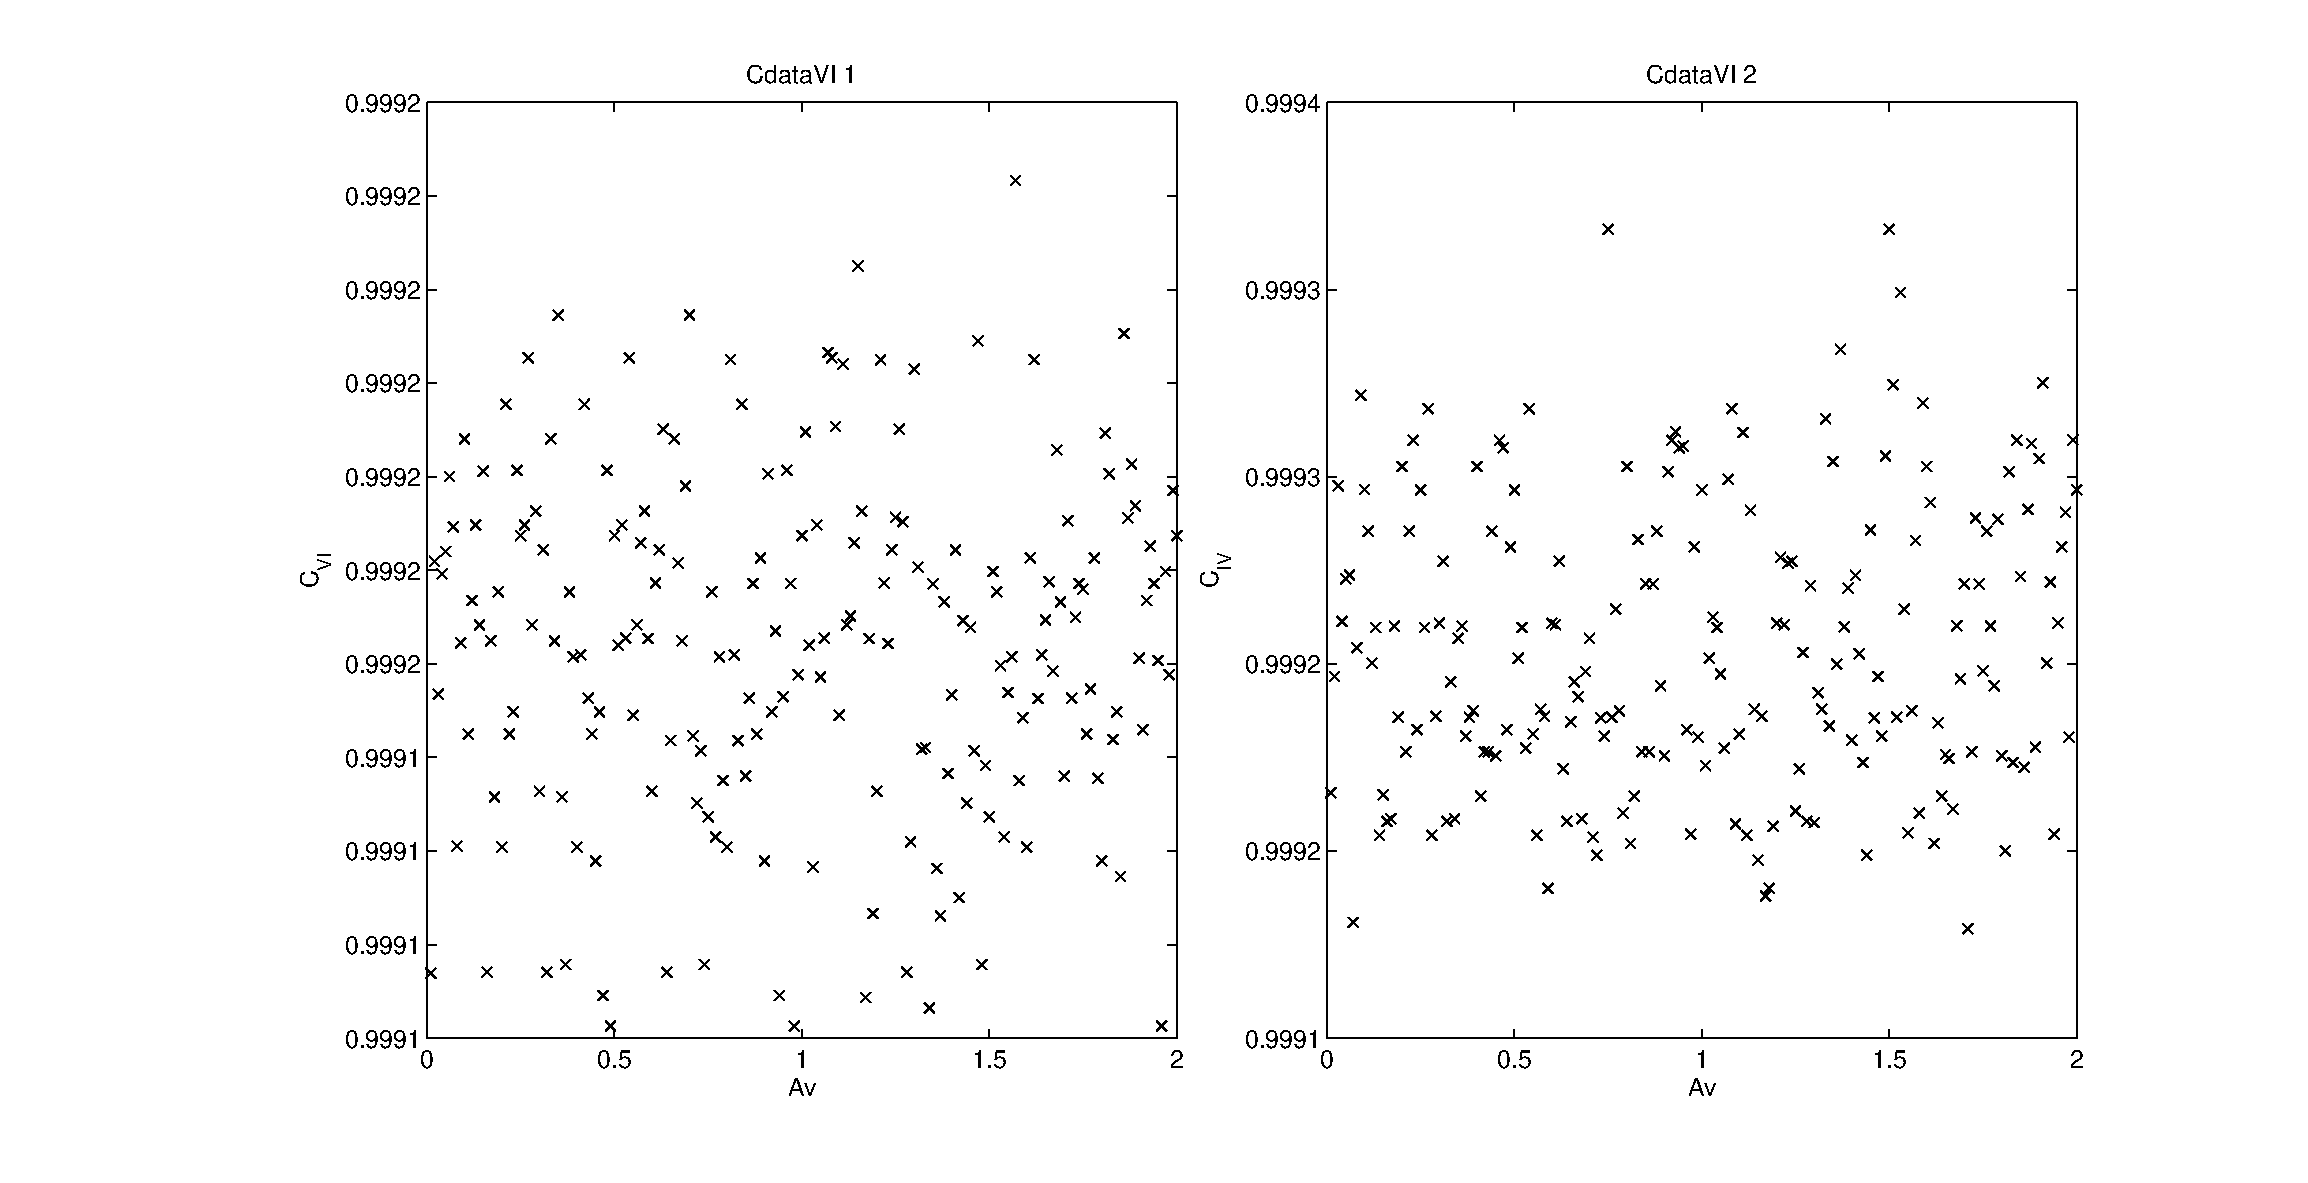
\includegraphics[scale=0.5]{RLCircuitPlots/RLcirc_varyV_amp2.eps} \\
(a) $C_{VI}$ and $C_{IV}$ \\[6pt]
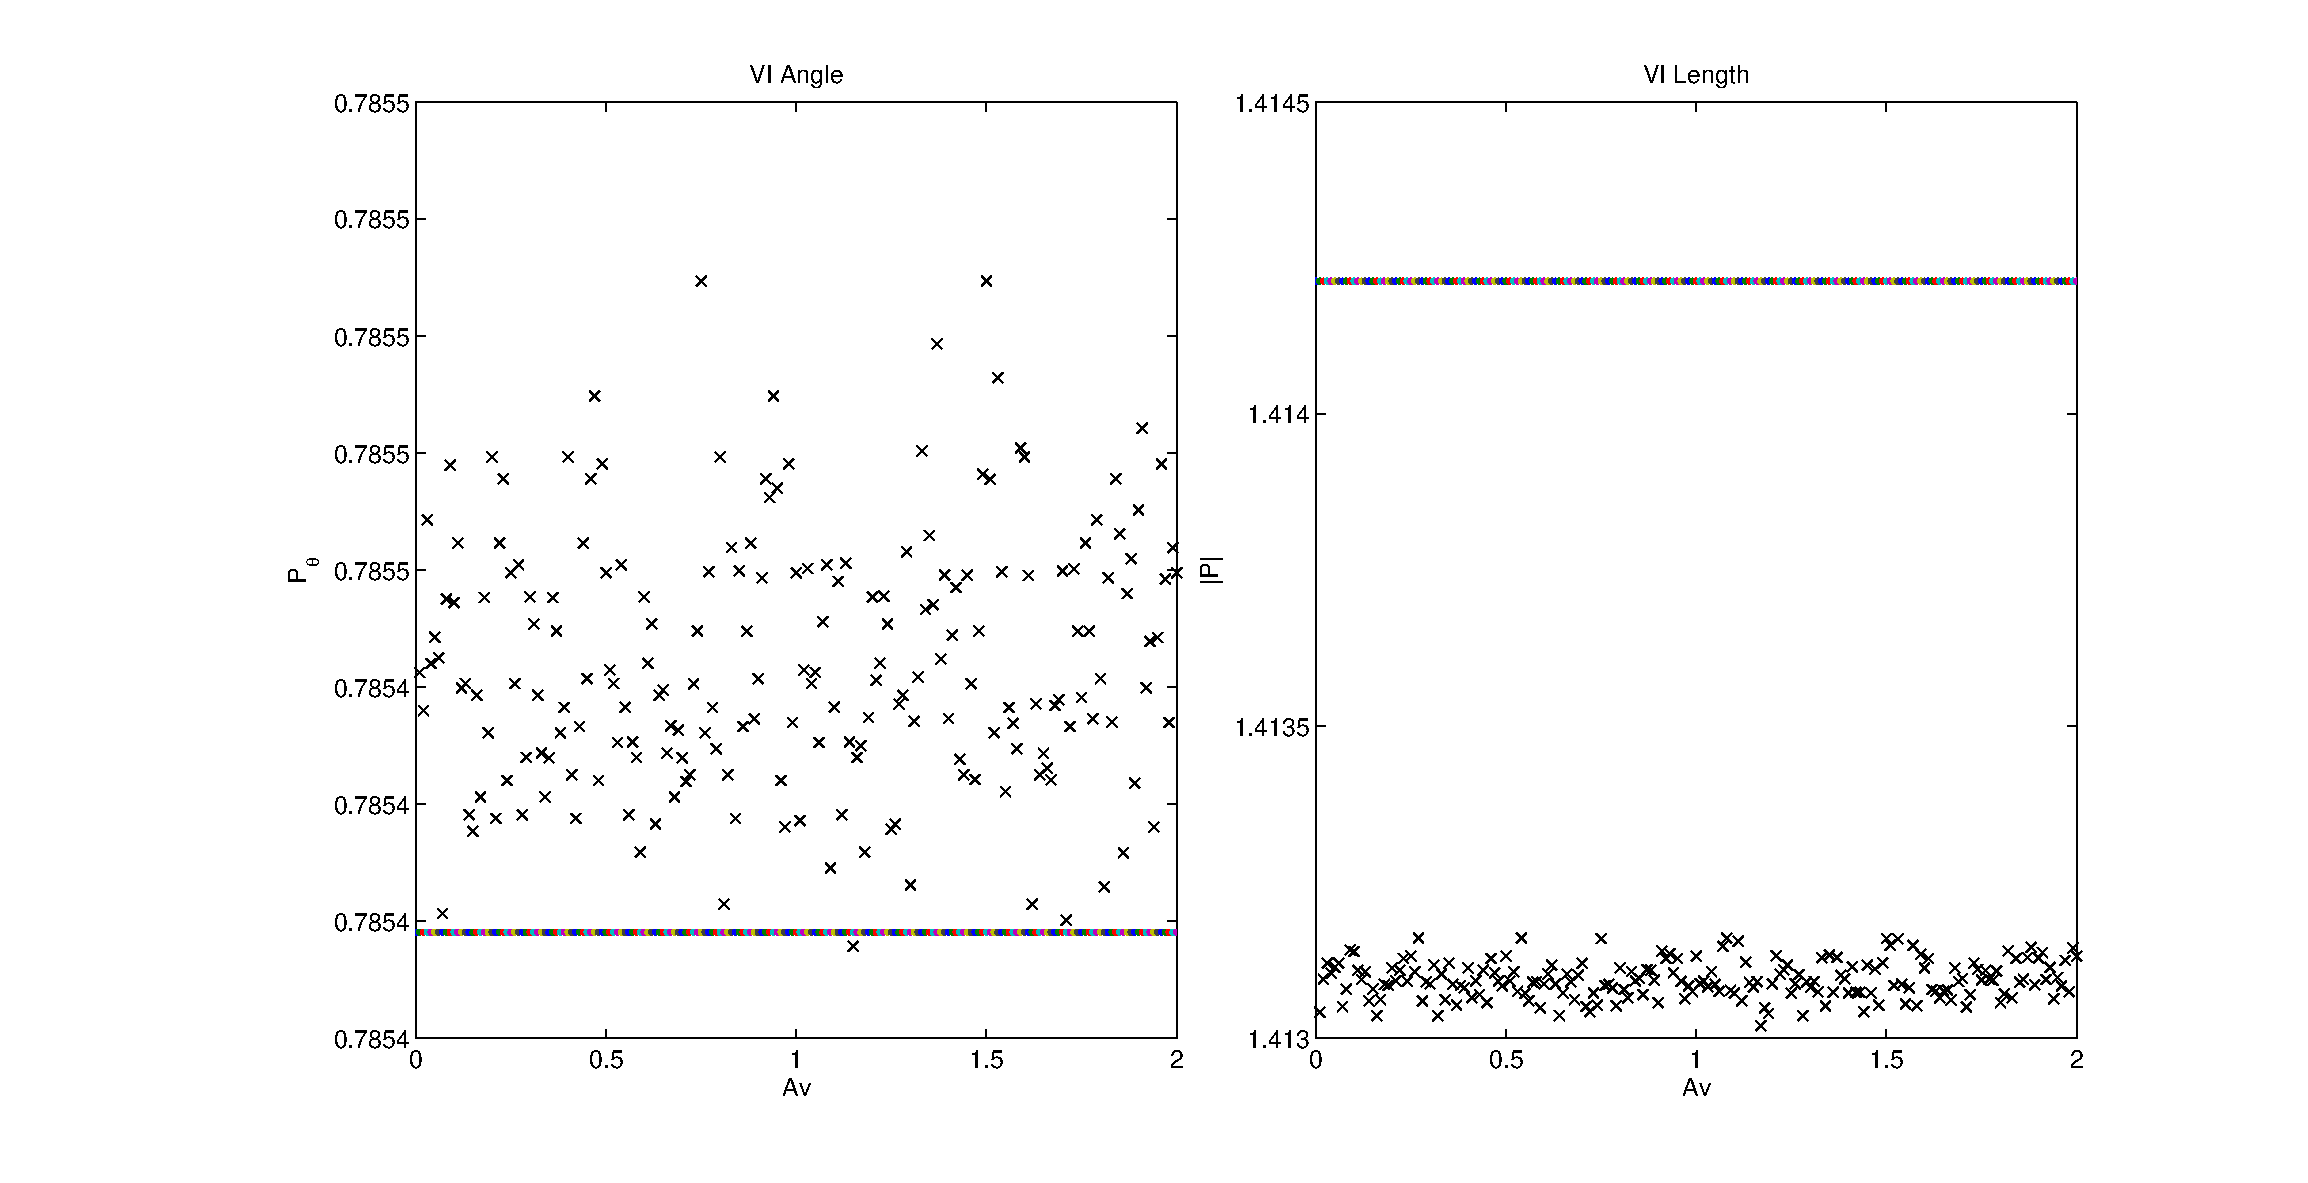
\includegraphics[scale=0.5]{RLCircuitPlots/RLcirc_varyV_amp.eps} \\
(b) $P_\theta$ and $|P|$ \\[6pt]
\end{tabular}
\caption{Changing $A_v$.}
\label{fig:Av}
\end{figure}

\subsection{Changing $f_v$}
Consider evaluating the CCM correlations $C_{VI}$ and $C_{IV}$ for each $f_v\in[0.01,2.0]$ in steps of $0.01$.  The CCM correlations are each plotted in Figure \ref{fig:fv} along with the corresponding PAI elements $P_\theta$ and $|P|$.
\begin{figure}[H]
\begin{tabular}{cc}
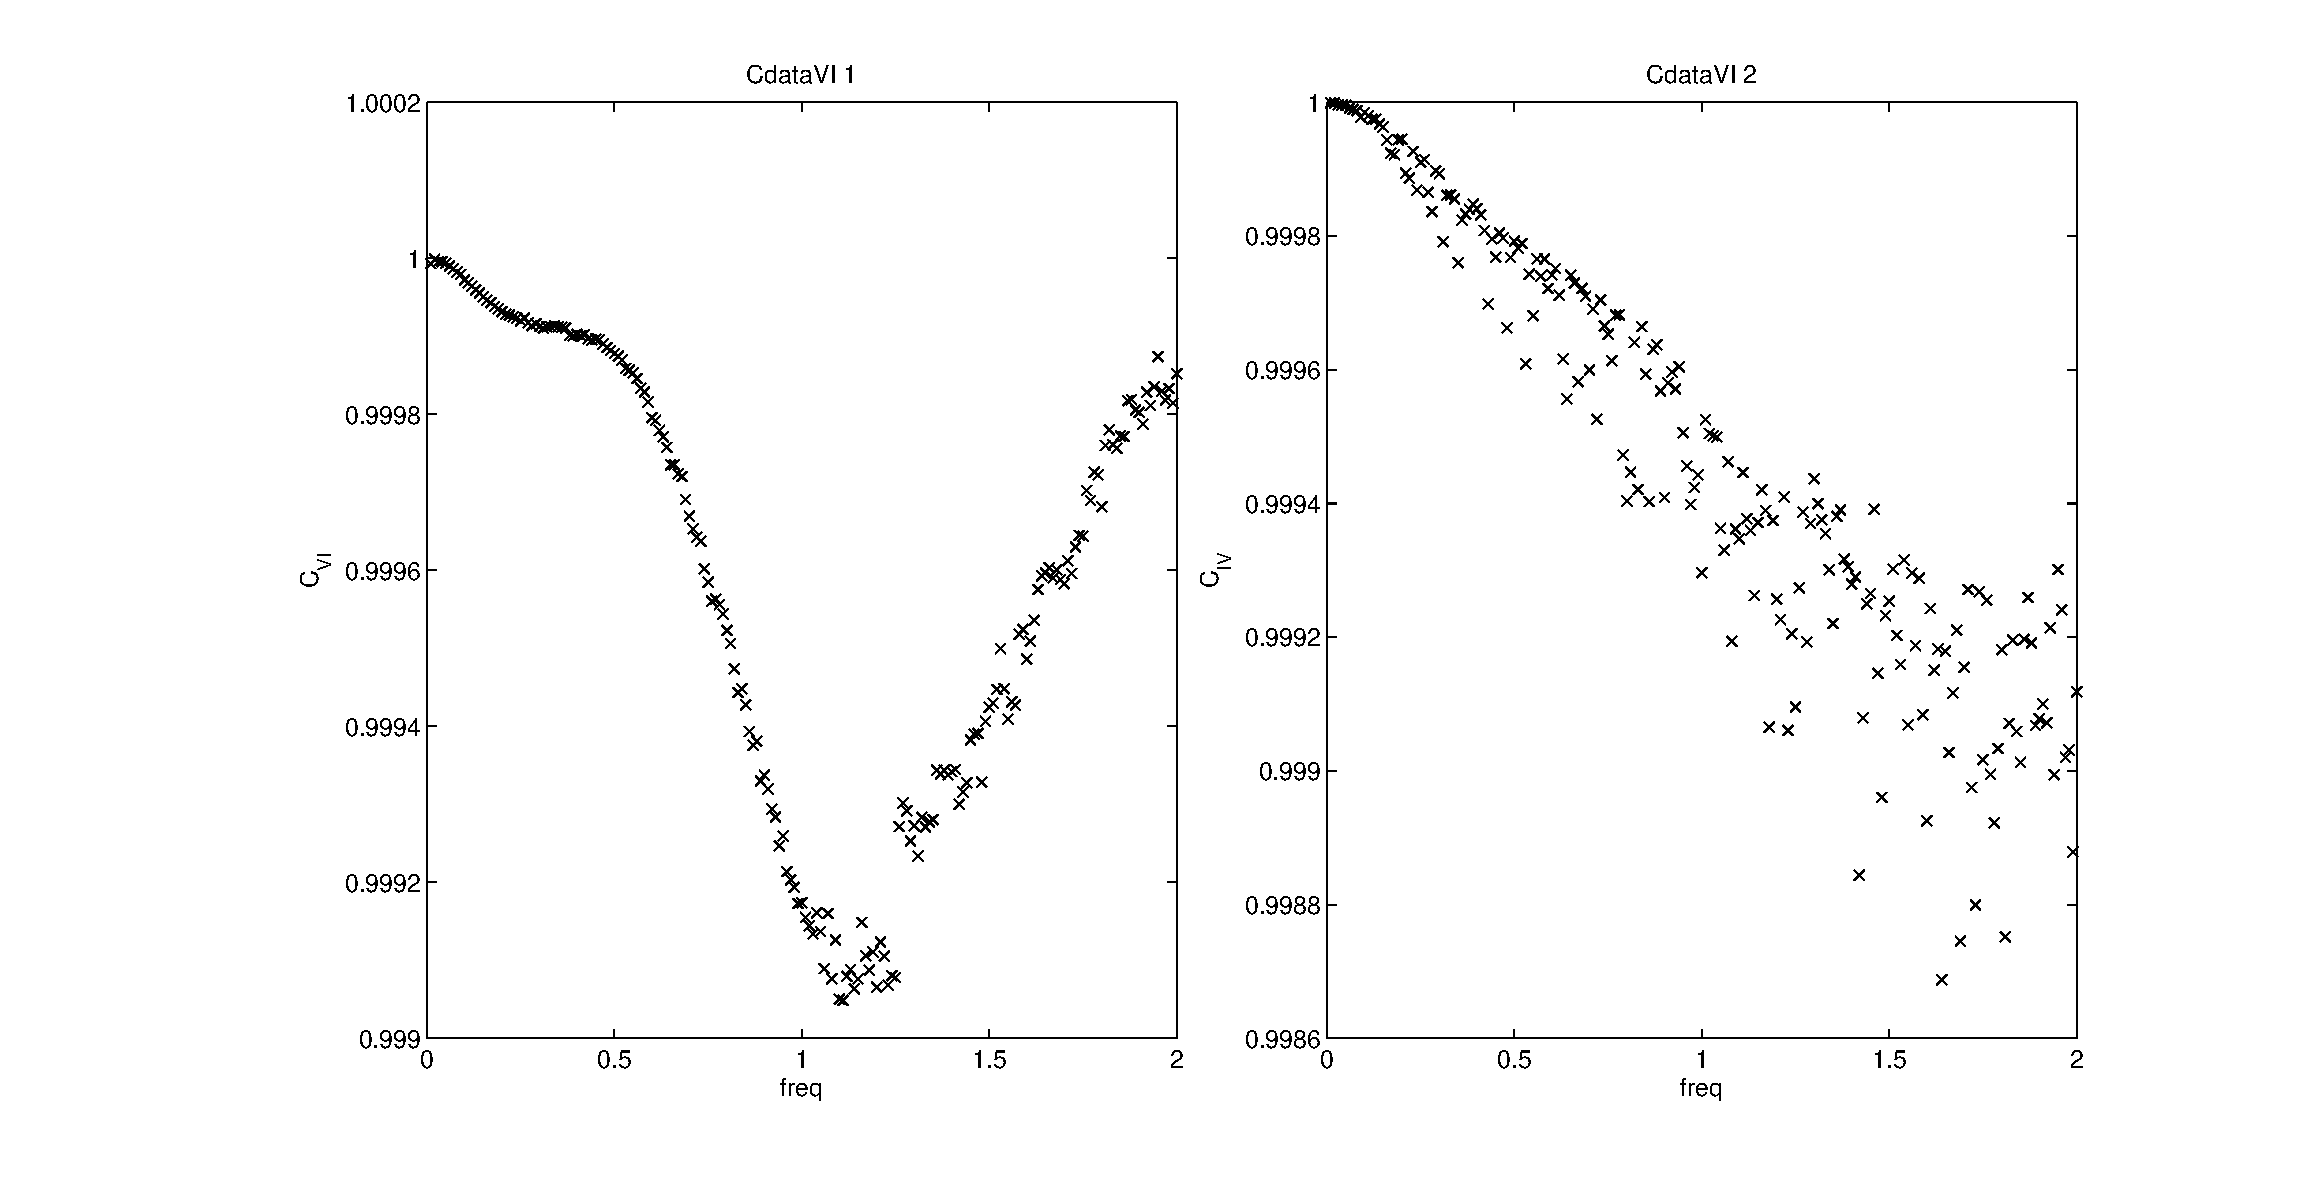
\includegraphics[scale=0.5]{RLCircuitPlots/RLcirc_varyV_freq2.eps} \\
(a) $C_{VI}$ and $C_{IV}$ \\[6pt]
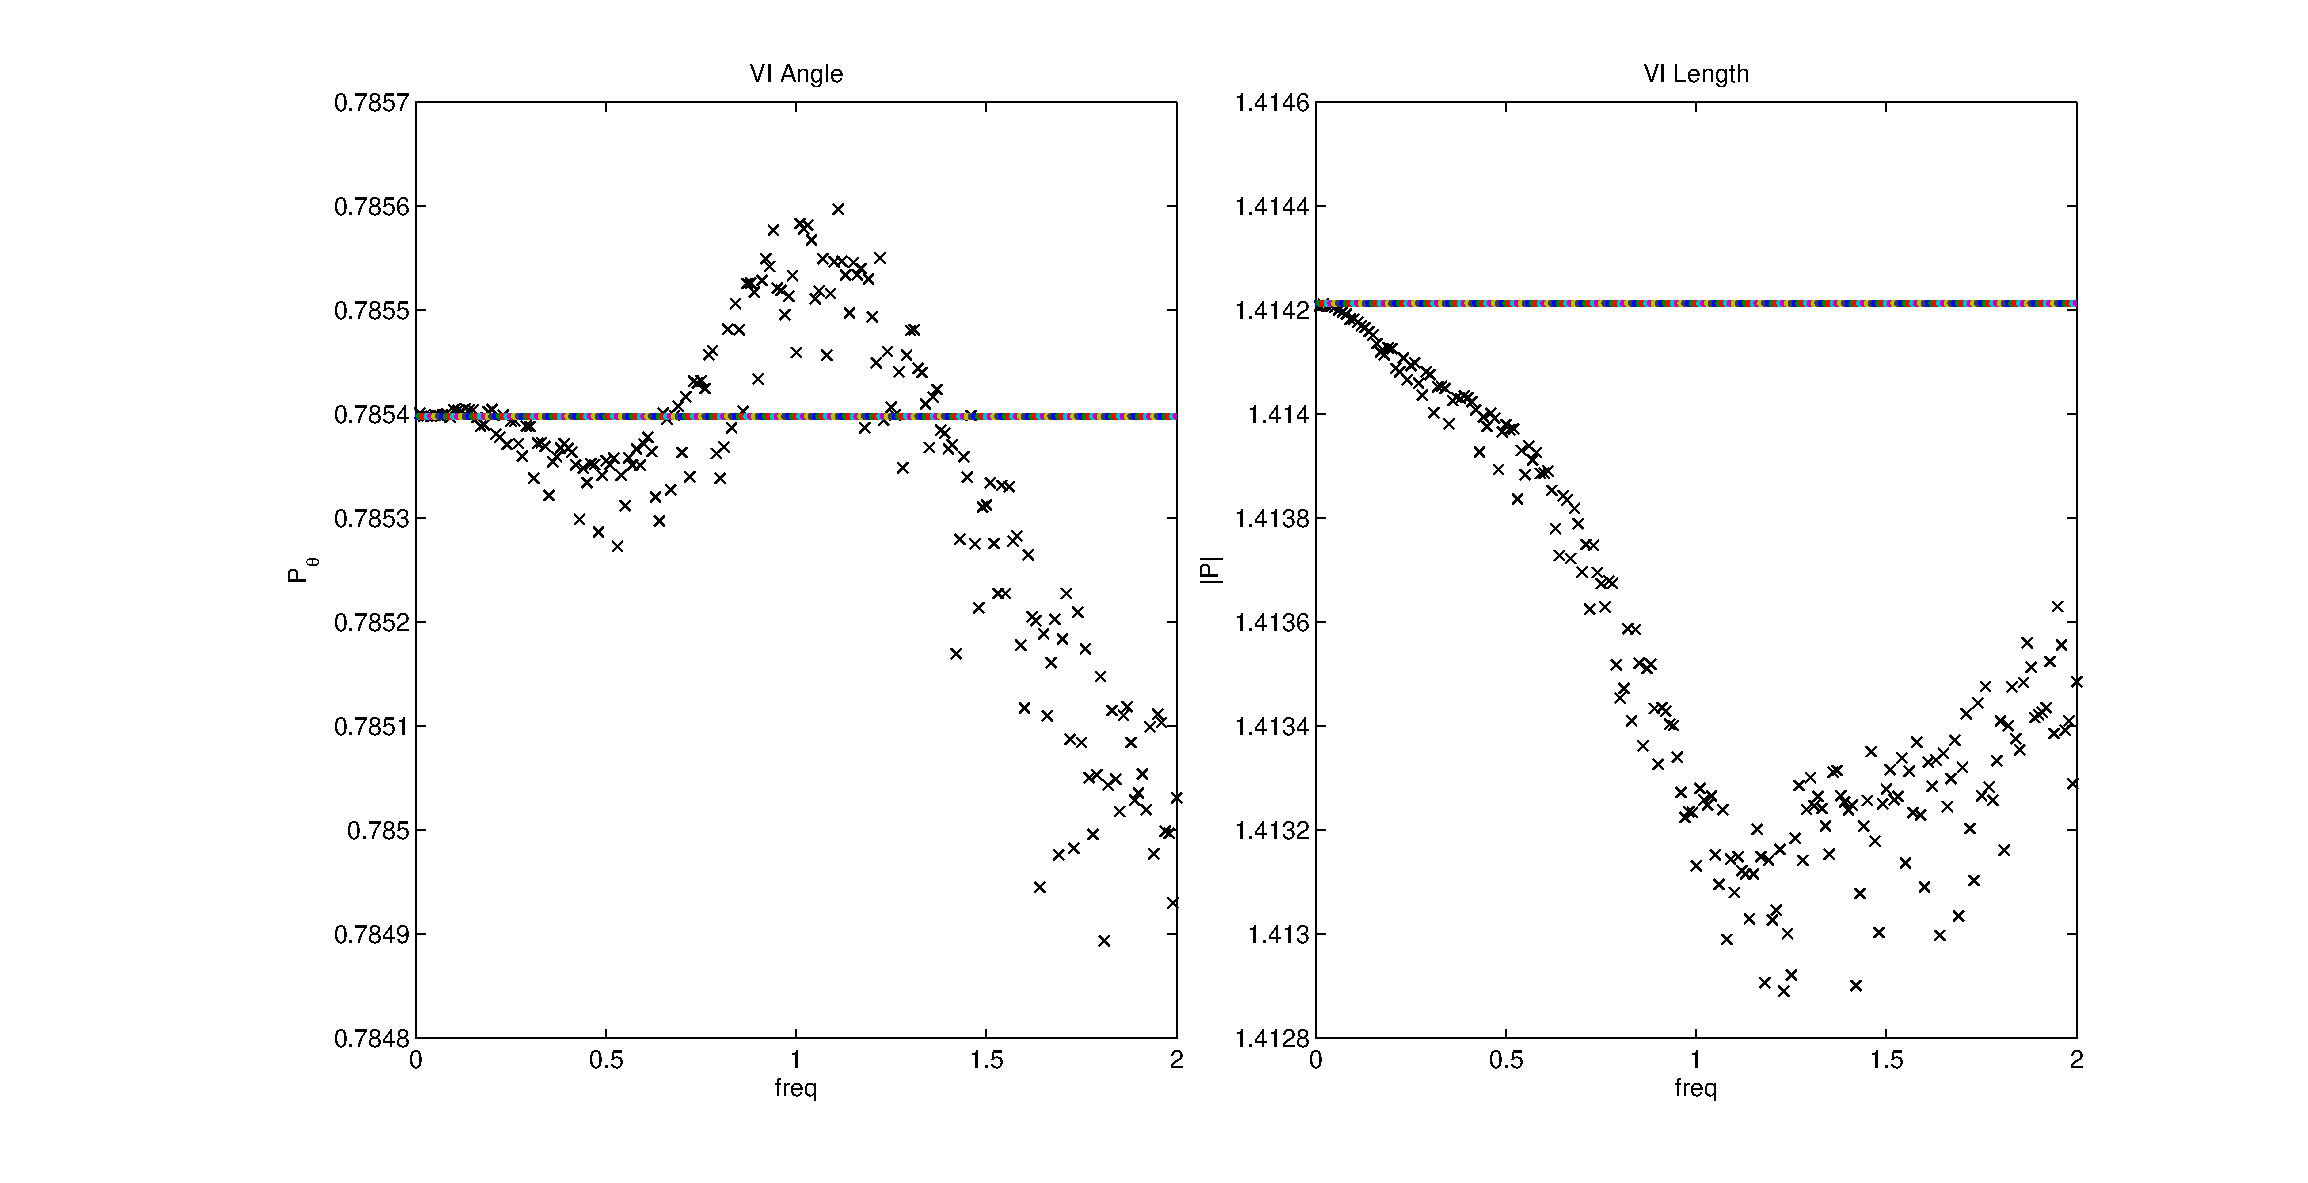
\includegraphics[scale=0.5]{RLCircuitPlots/RLcirc_varyV_freq.eps} \\
(b) $P_\theta$ and $|P|$ \\[6pt]
\end{tabular}
\caption{Changing $f_v$.}
\label{fig:fv}
\end{figure}

\subsection{Changing $\phi_v$}
Consider evaluating the CCM correlations $C_{VI}$ and $C_{IV}$ for each $\phi_v\in[0.01,2.0]$ in steps of $0.01$.  The CCM correlations are each plotted in Figure \ref{fig:Pv} along with the corresponding PAI elements $P_\theta$ and $|P|$.
\begin{figure}[H]
\begin{tabular}{cc}
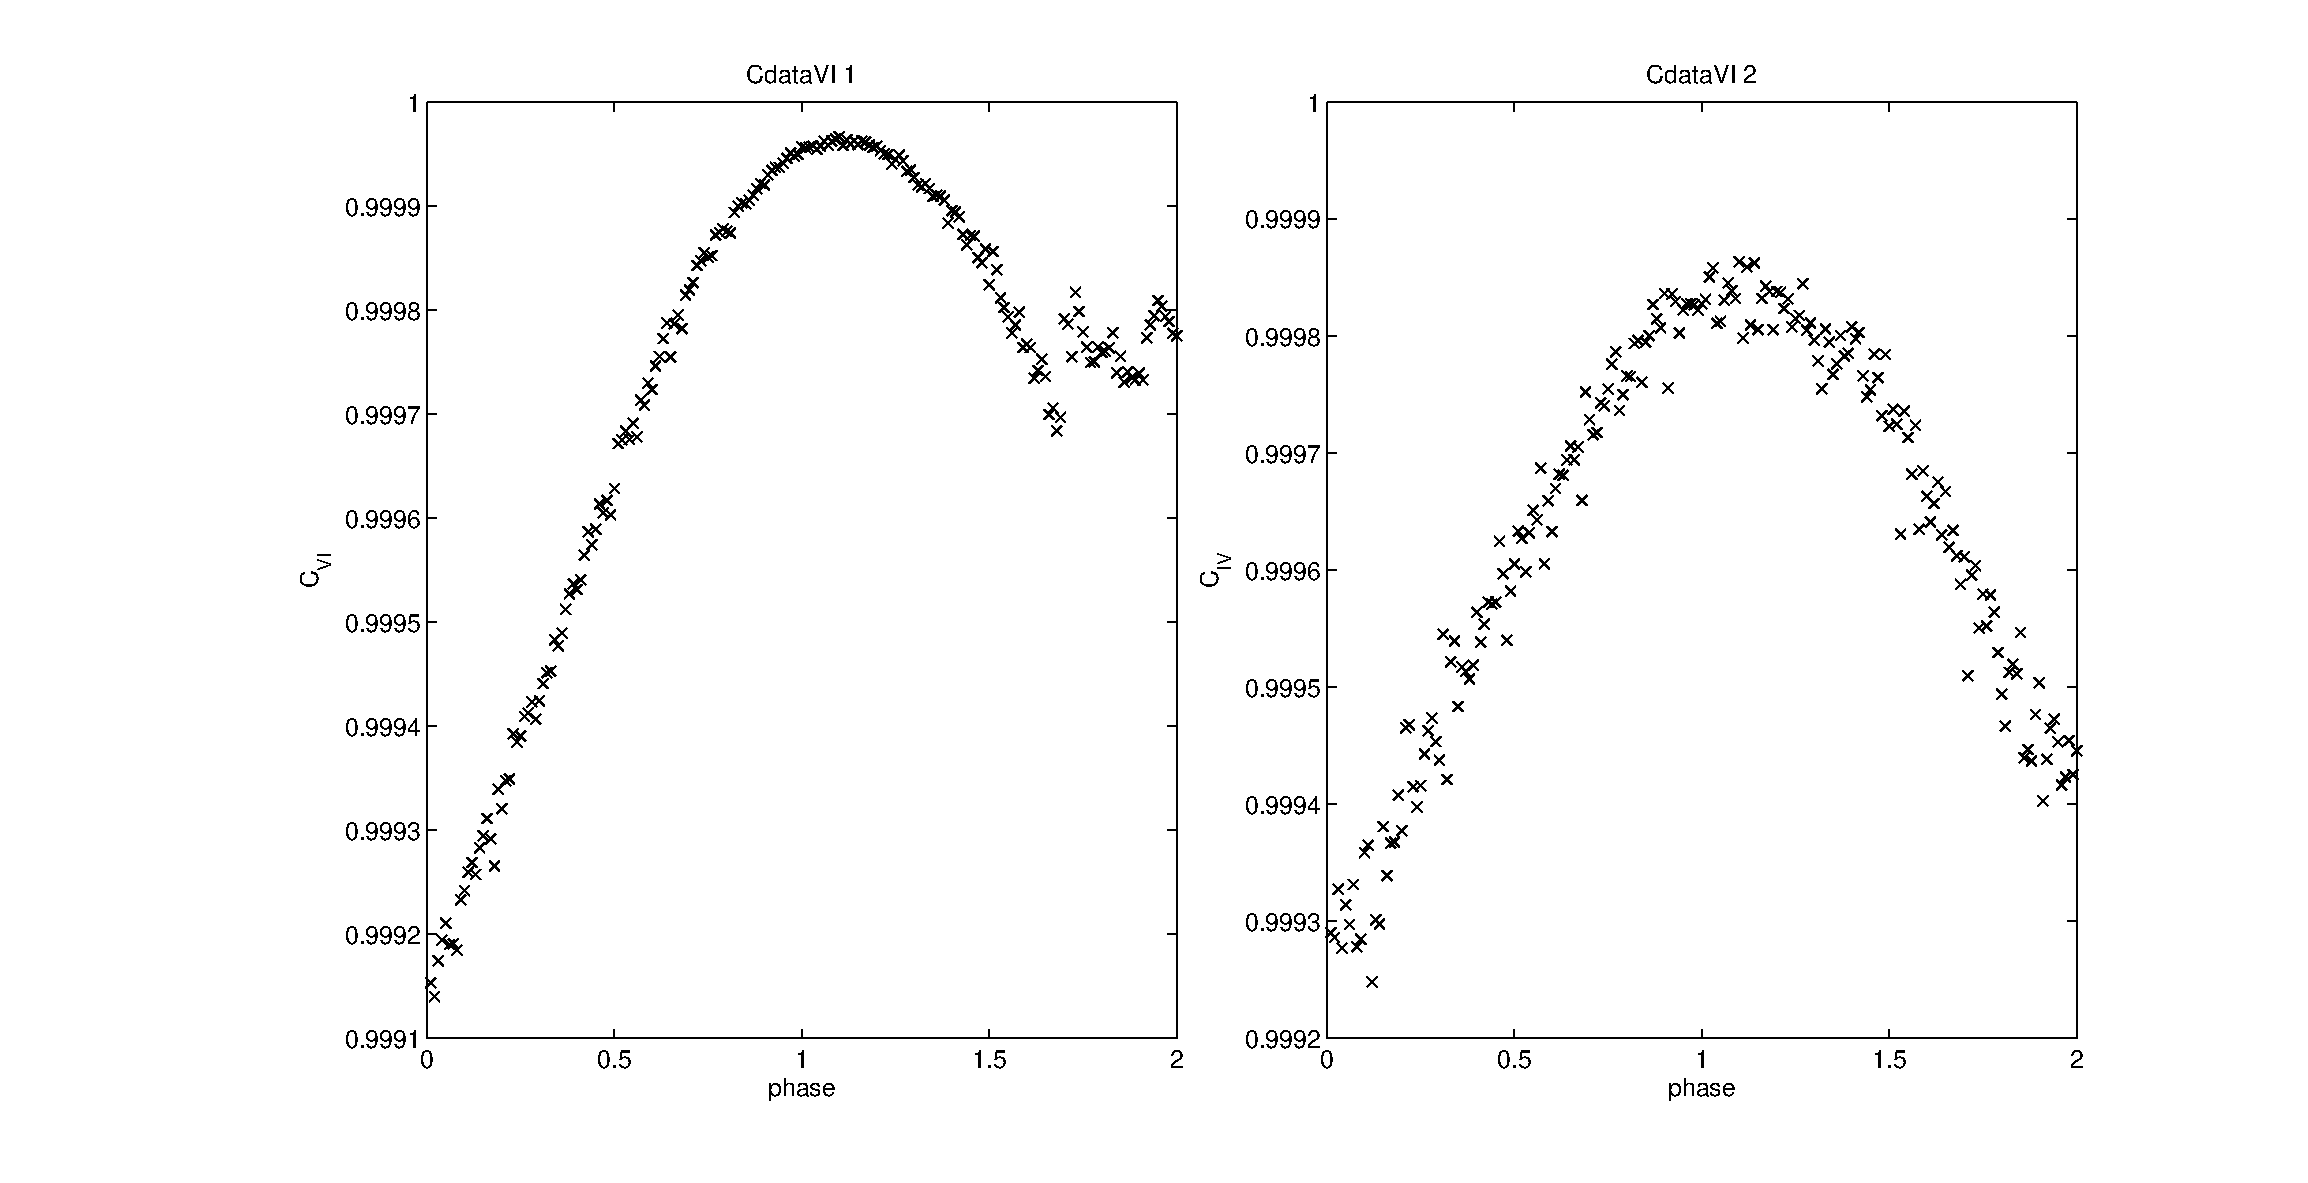
\includegraphics[scale=0.5]{RLCircuitPlots/RLcirc_varyV_phase2.eps} \\
(a) $C_{VI}$ and $C_{IV}$ \\[6pt]
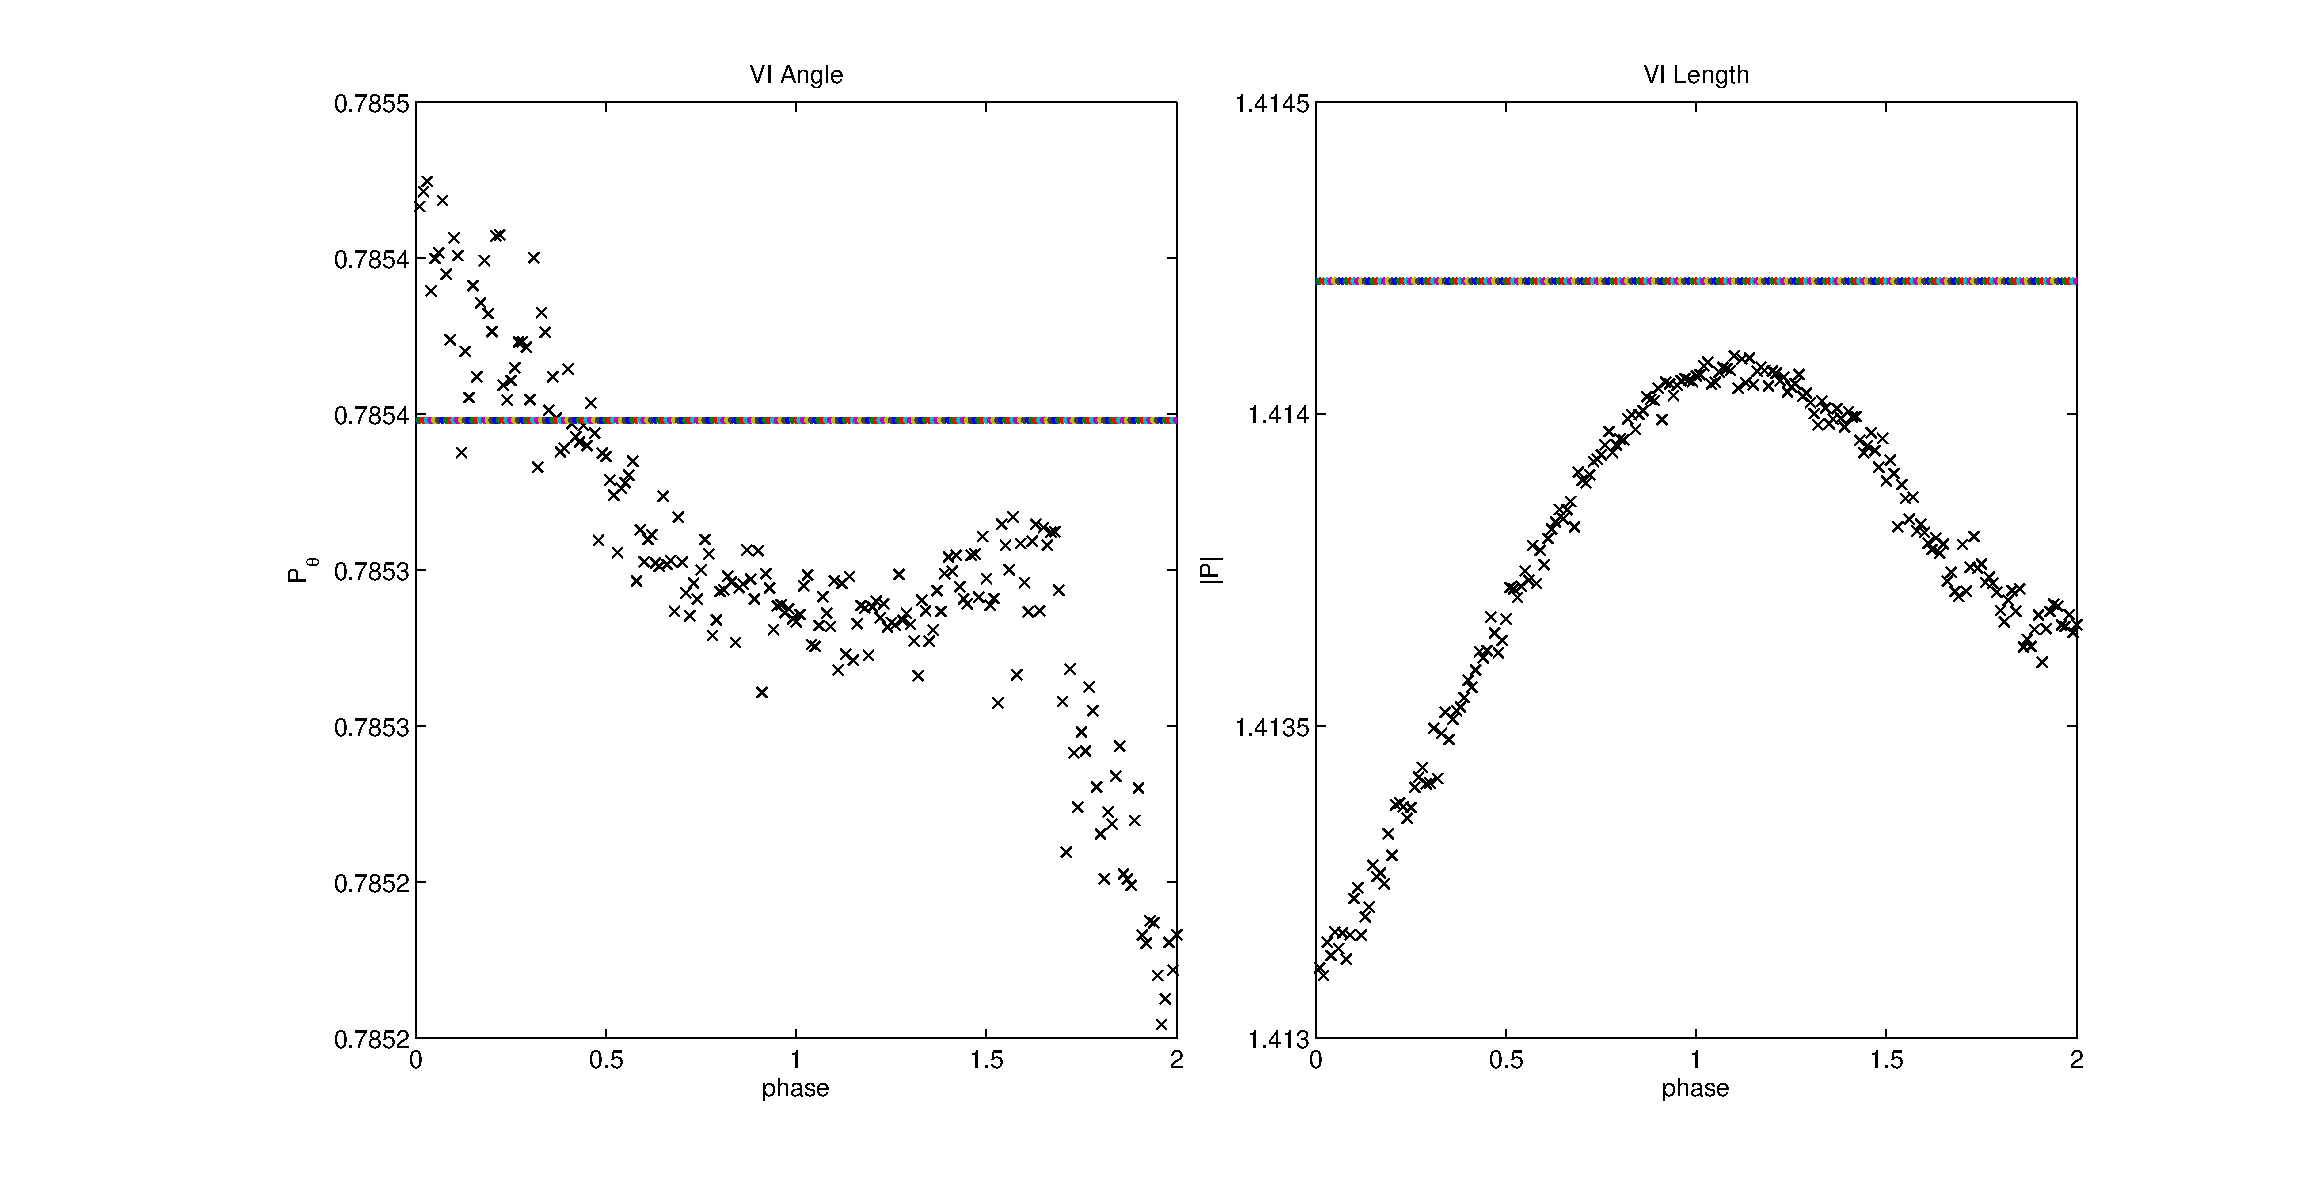
\includegraphics[scale=0.5]{RLCircuitPlots/RLcirc_varyV_phase.eps} \\
(b) $P_\theta$ and $|P|$ \\[6pt]
\end{tabular}
\caption{Changing $\phi_v$.}
\label{fig:Pv}
\end{figure}

\subsection{Changing $O_v$}
Consider evaluating the CCM correlations $C_{VI}$ and $C_{IV}$ for each $O_v\in[0.01,2.0]$ in steps of $0.01$.  The CCM correlations are each plotted in Figure \ref{fig:Ov} along with the corresponding PAI elements $P_\theta$ and $|P|$.
\begin{figure}[H]
\begin{tabular}{cc}
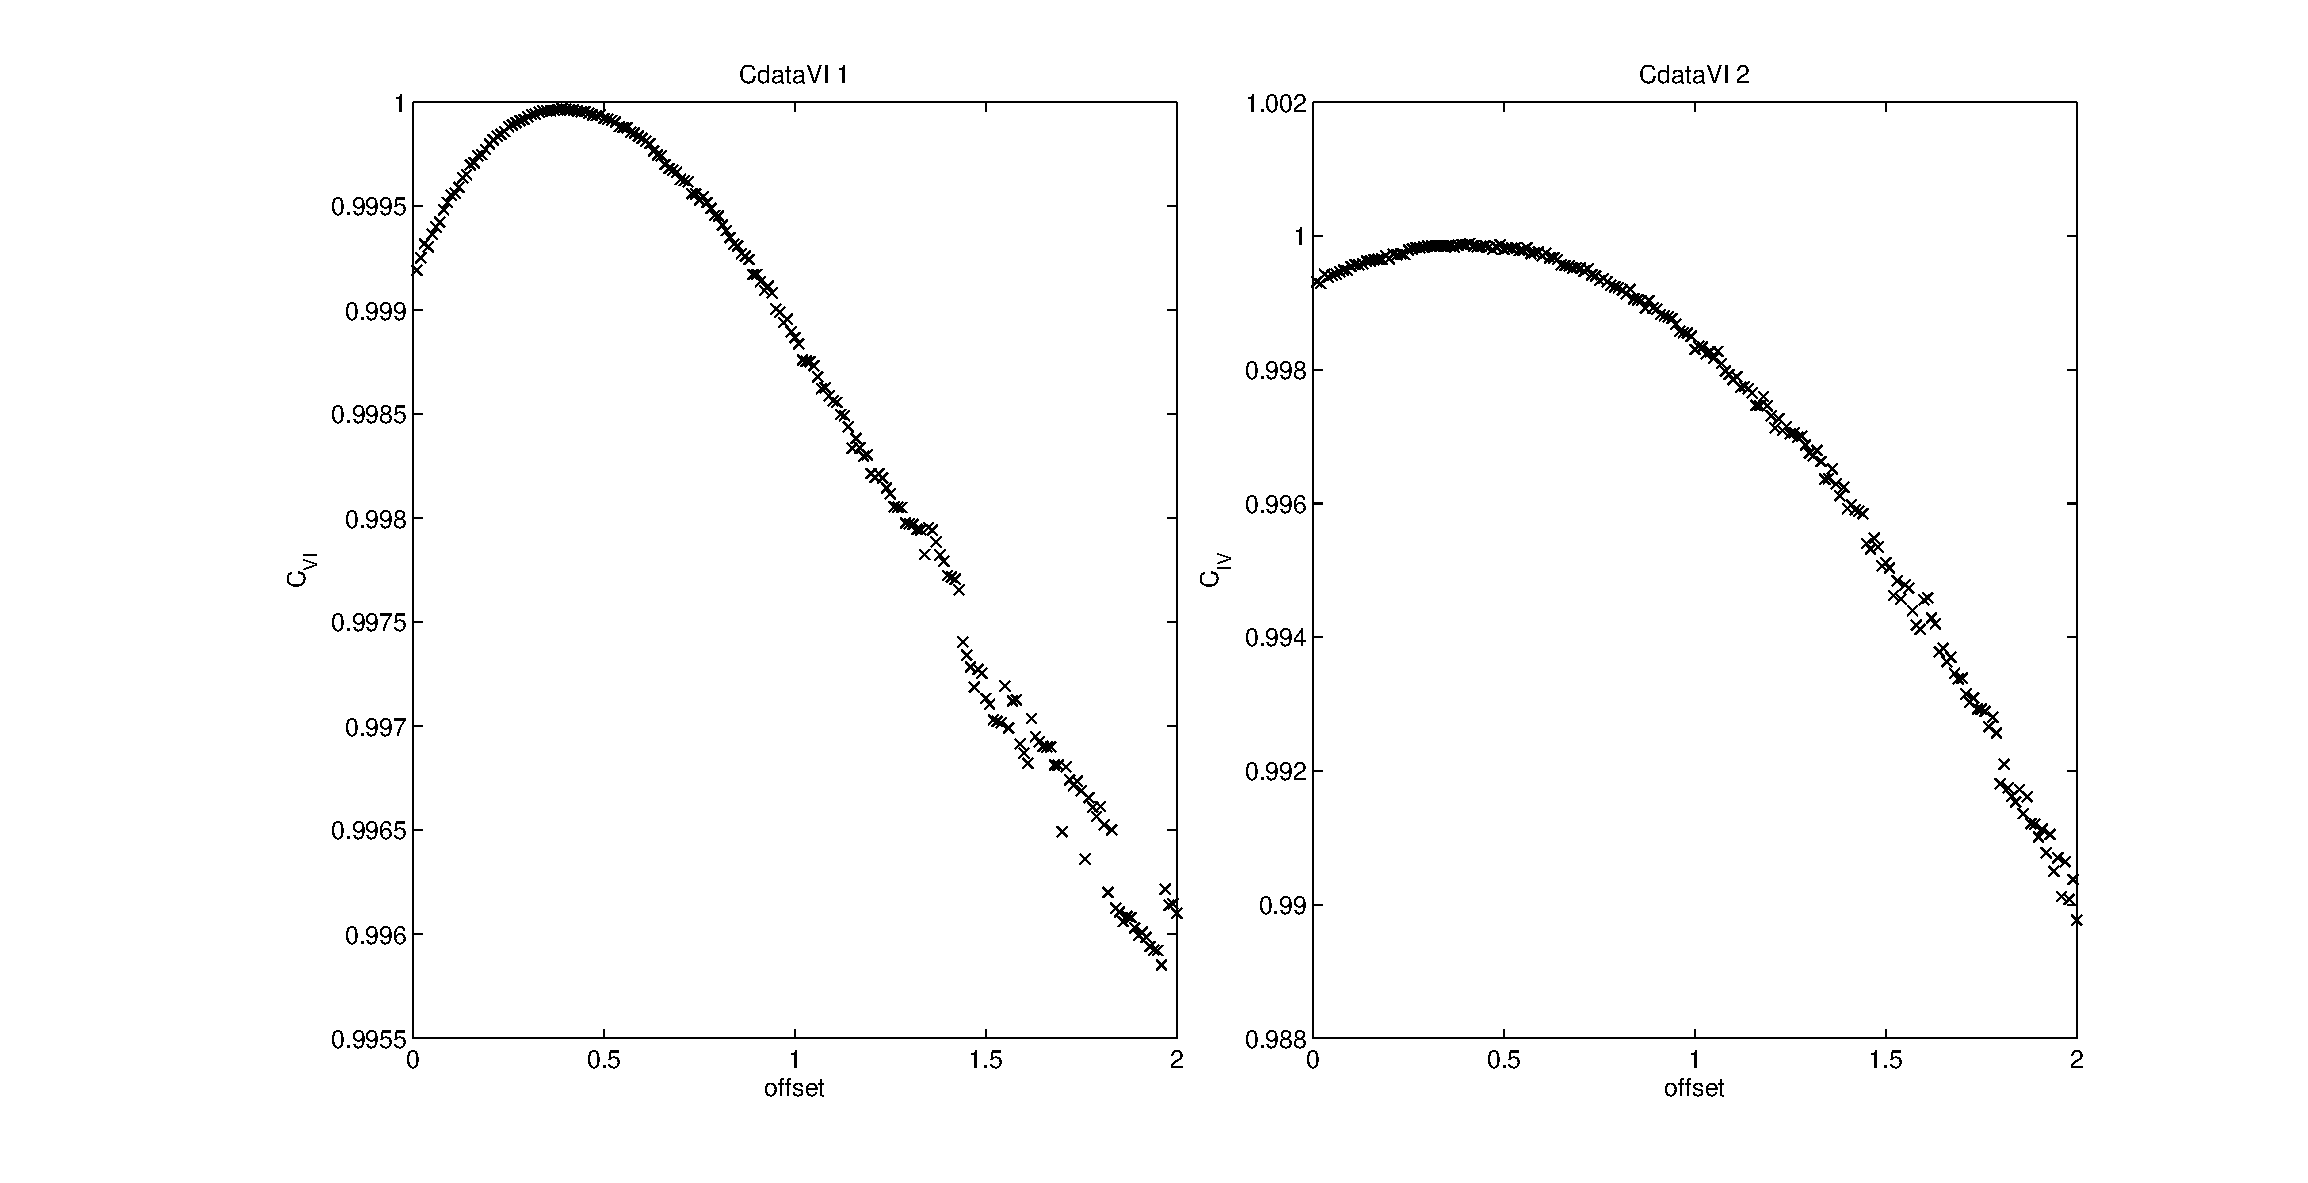
\includegraphics[scale=0.5]{RLCircuitPlots/RLcirc_varyV_offset2.eps} \\
(a) $C_{VI}$ and $C_{IV}$ \\[6pt]
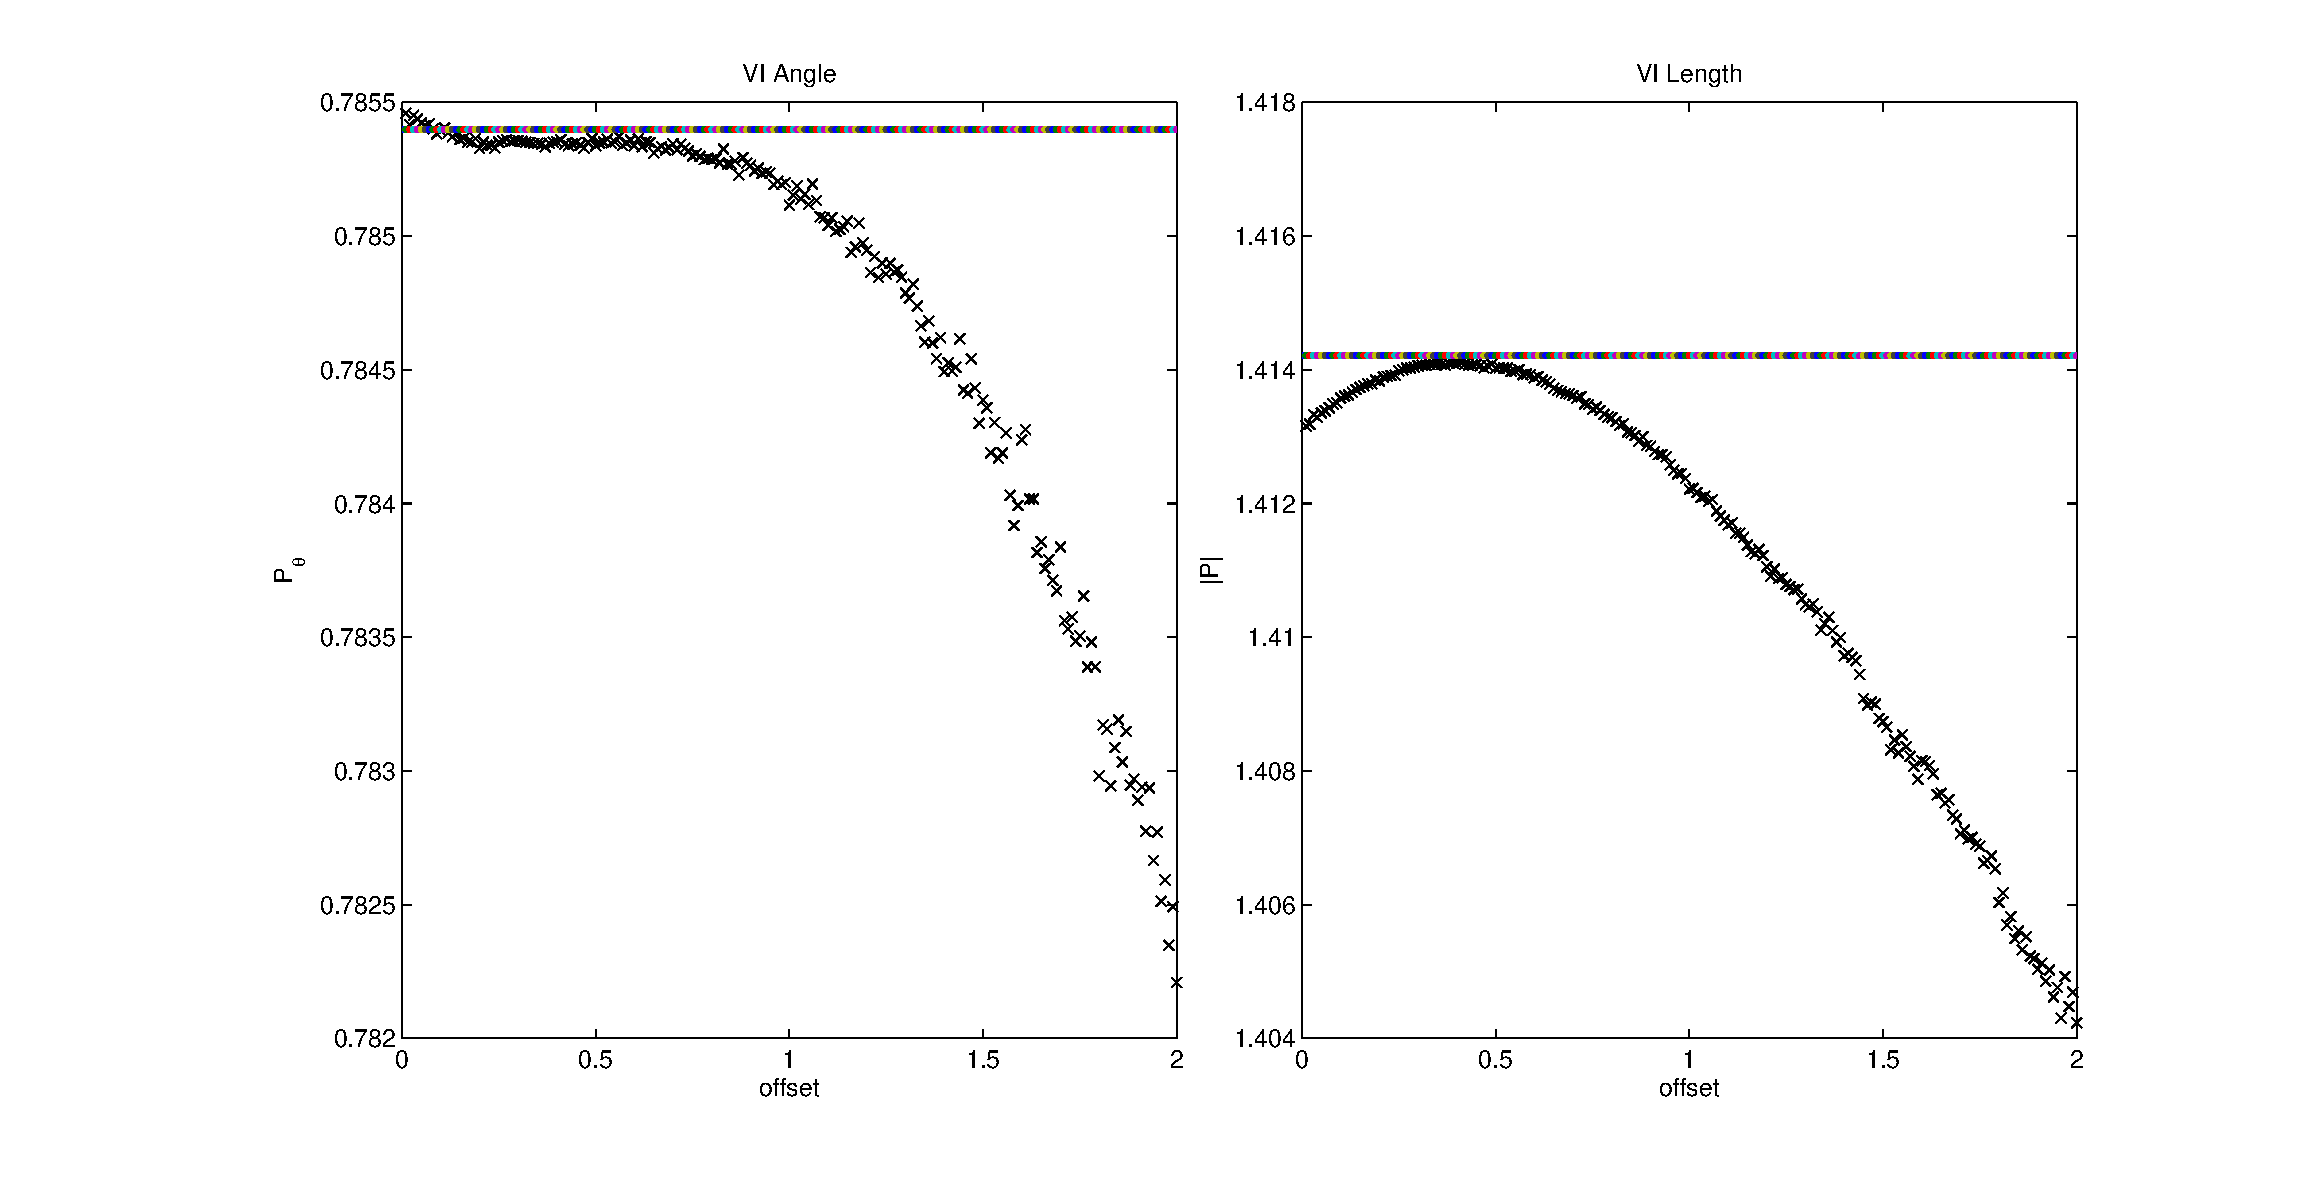
\includegraphics[scale=0.5]{RLCircuitPlots/RLcirc_varyV_offset.eps} \\
(b) $P_\theta$ and $|P|$ \\[6pt]
\end{tabular}
\caption{Changing $O_v$.}
\label{fig:Ov}
\end{figure}

Figure \ref{fig:Ov1} shows the effect of increasing the library length from $2\times10^3$ (i.e.\ {\tt tspan = [0:0.5:1000];}) to $10^4$ (i.e.\ {\tt tspan = [0:0.5:5000];}), and Figure \ref{fig:Ov2} extends the above plots to $O_v\in[0.01,10.0]$ in steps of $0.05$.
\begin{figure}[H]
\begin{tabular}{cc}
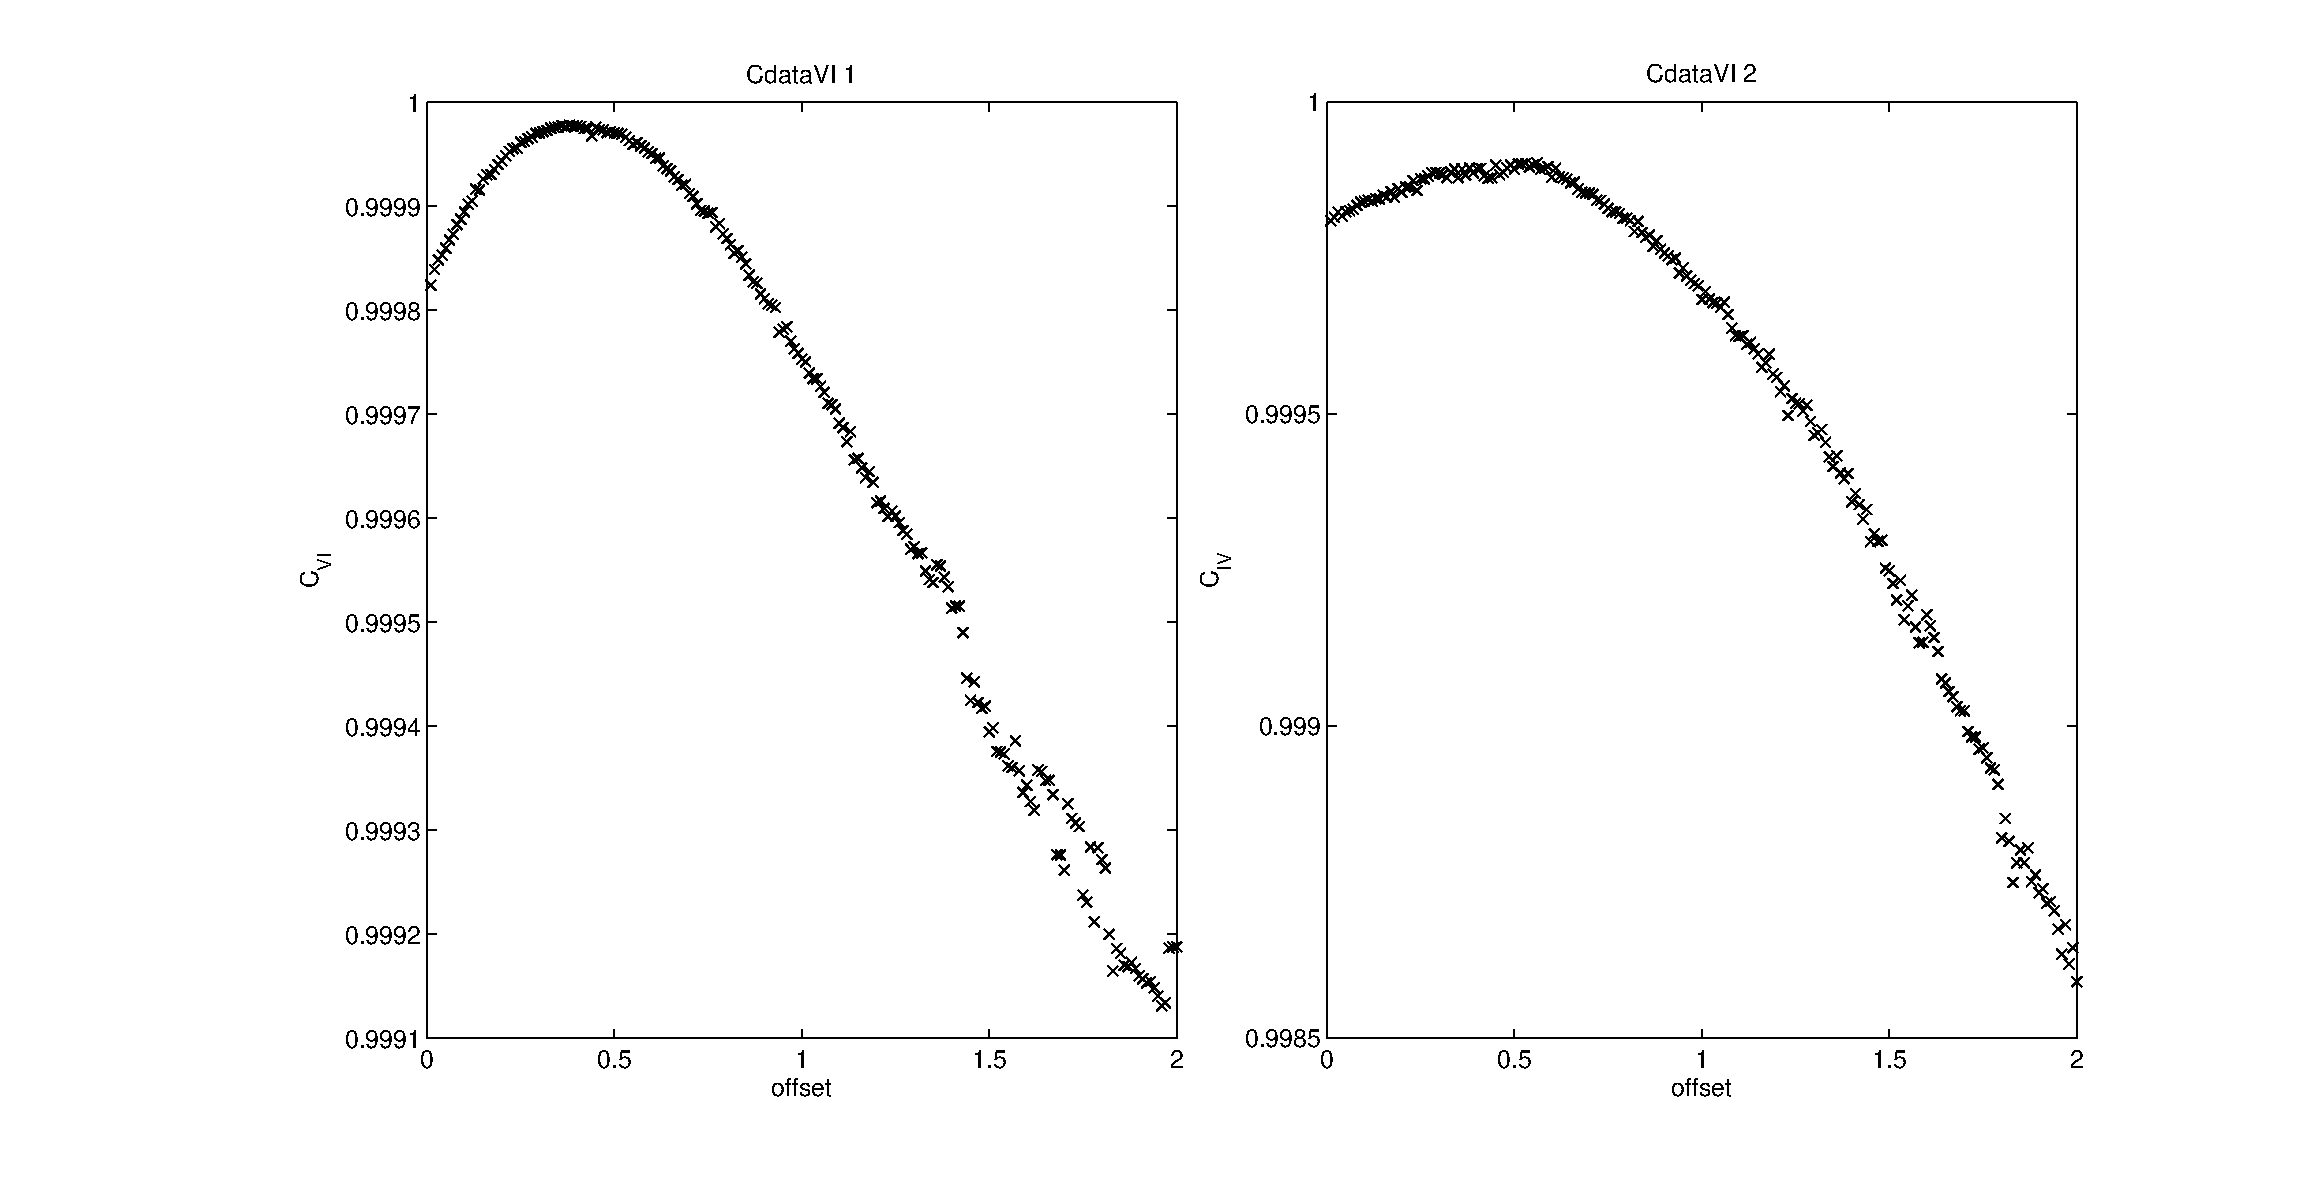
\includegraphics[scale=0.5]{RLCircuitPlots/RLcirc_varyV_offsetLup2.eps} \\
(a) $C_{VI}$ and $C_{IV}$ \\[6pt]
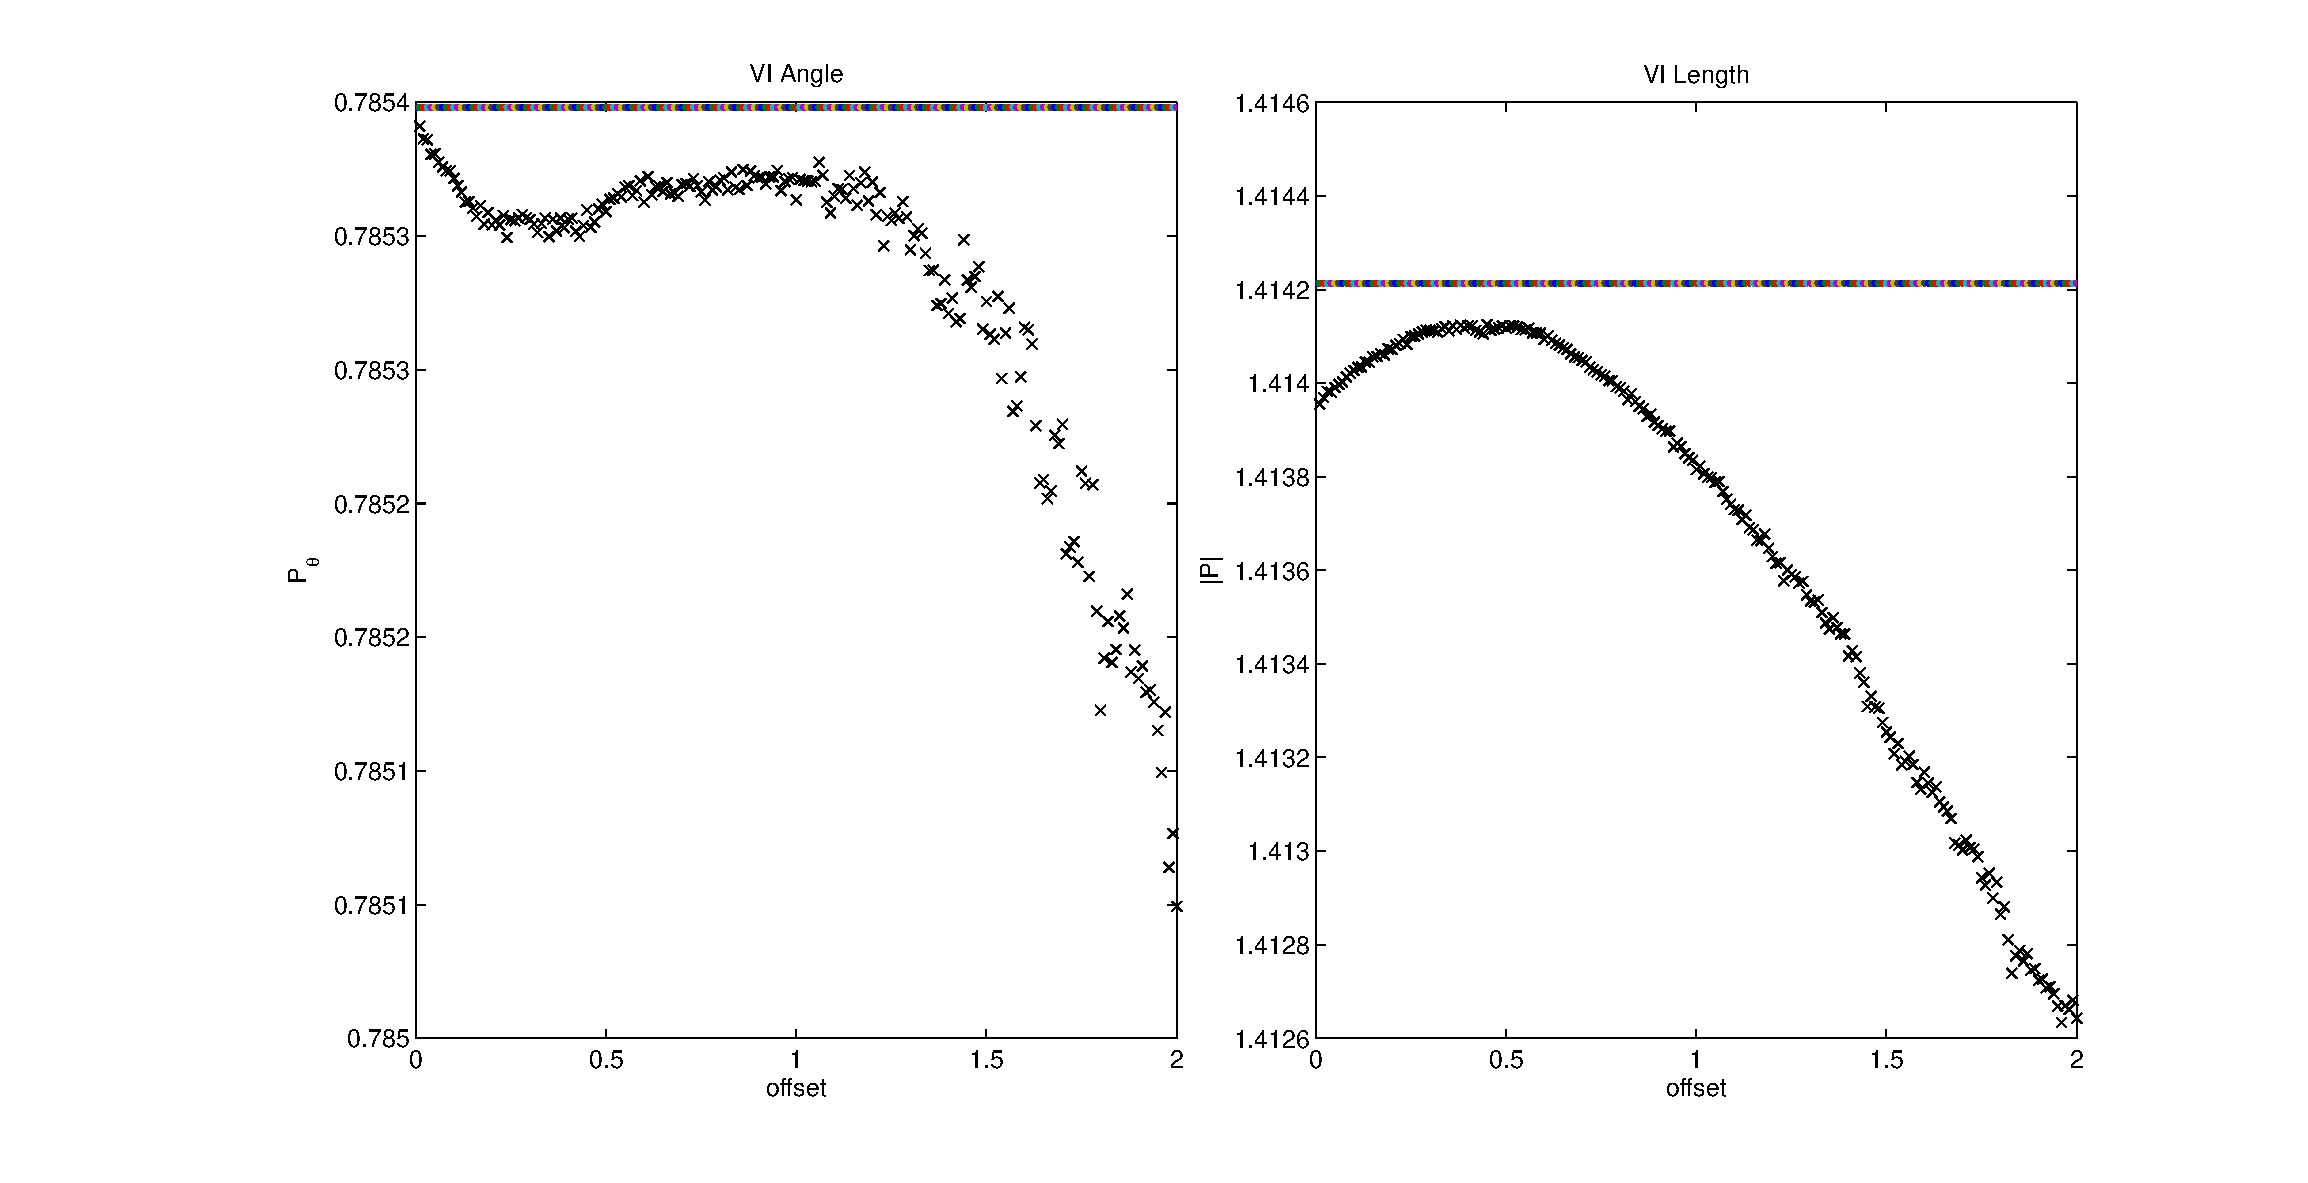
\includegraphics[scale=0.5]{RLCircuitPlots/RLcirc_varyV_offsetLup.eps} \\
(b) $P_\theta$ and $|P|$ \\[6pt]
\end{tabular}
\caption{Changing $O_v$ (longer library length).}
\label{fig:Ov1}
\end{figure}
\begin{figure}[H]
\begin{tabular}{cc}
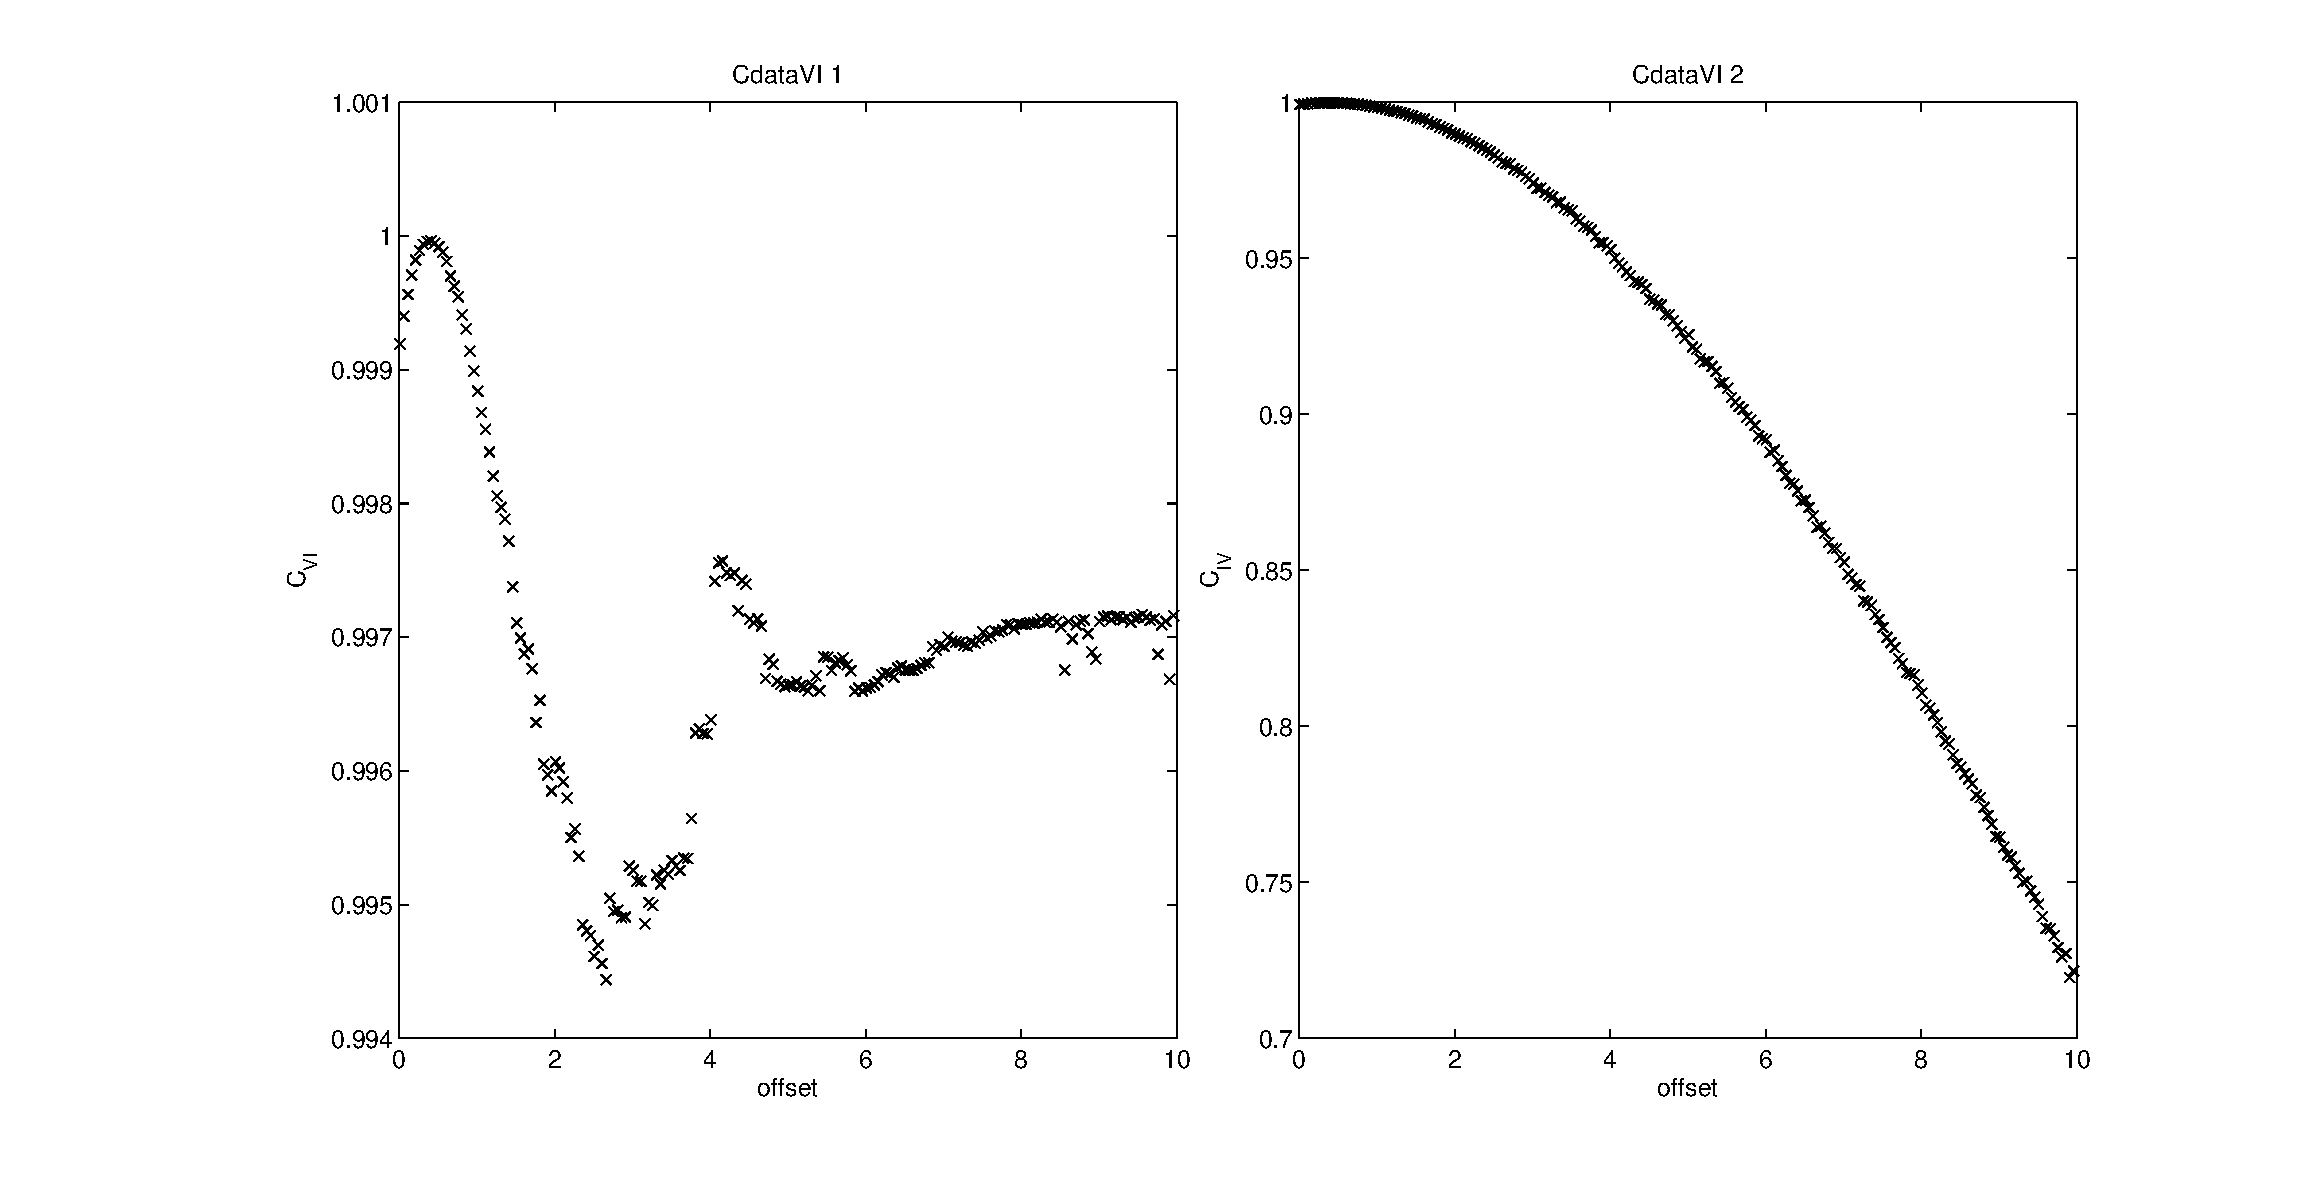
\includegraphics[scale=0.5]{RLCircuitPlots/RLcirc_varyV_offsetlong2.eps} \\
(a) $C_{VI}$ and $C_{IV}$ \\[6pt]
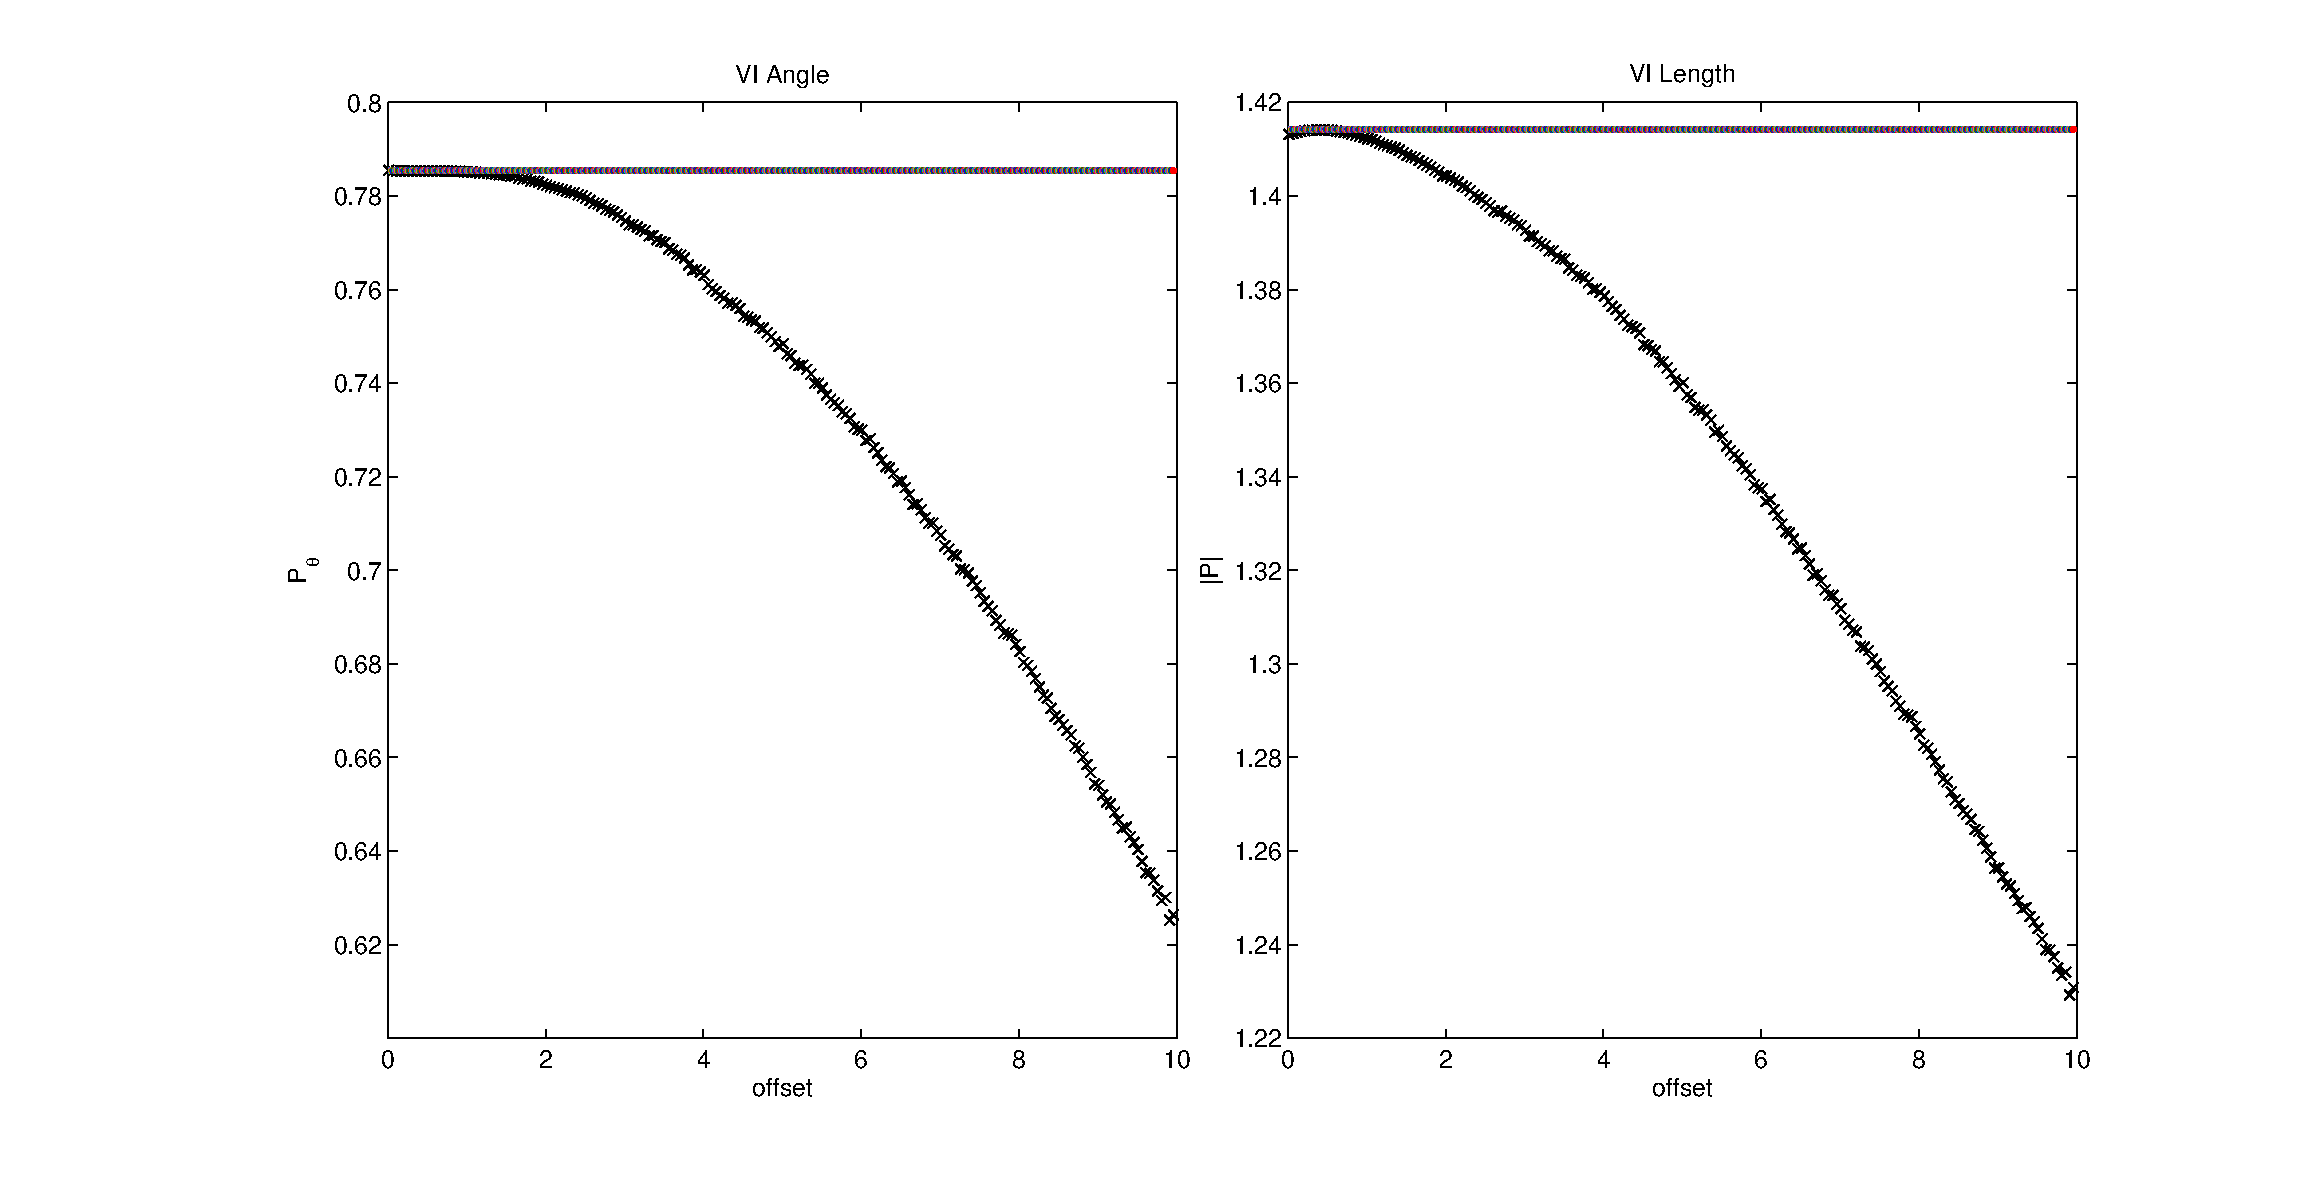
\includegraphics[scale=0.5]{RLCircuitPlots/RLcirc_varyV_offsetlong.eps} \\
(c) $P_\theta$ and $|P|$ \\[6pt]
\end{tabular}
\caption{Changing $O_v$ (larger domain for $O_v$).}
\label{fig:Ov2}
\end{figure}

\section{PAI}
Consider the system (Sugihara Figure 3 C and D)
\begin{eqnarray}
X_{t+1} &=& X_t\left(r_x-r_xX_t-\beta_{xy}Y_t\right)\\
Y_{t+1} &=& Y_t\left(r_y-r_yY_t-\beta_{yx}X_t\right),
\end{eqnarray}
with $r_y=r_y=3.7$, $X_0 = 0.2$, $Y_0=0.4$, $\beta_{xy}=0$, and $\beta_{yx}=0.32$.  Plots of the correlation between $X$ and $X|Y$, as well as, $Y$ and $Y|X$ are shown below.
\begin{center}
\begin{figure}[H]
\begin{tabular}{cc}
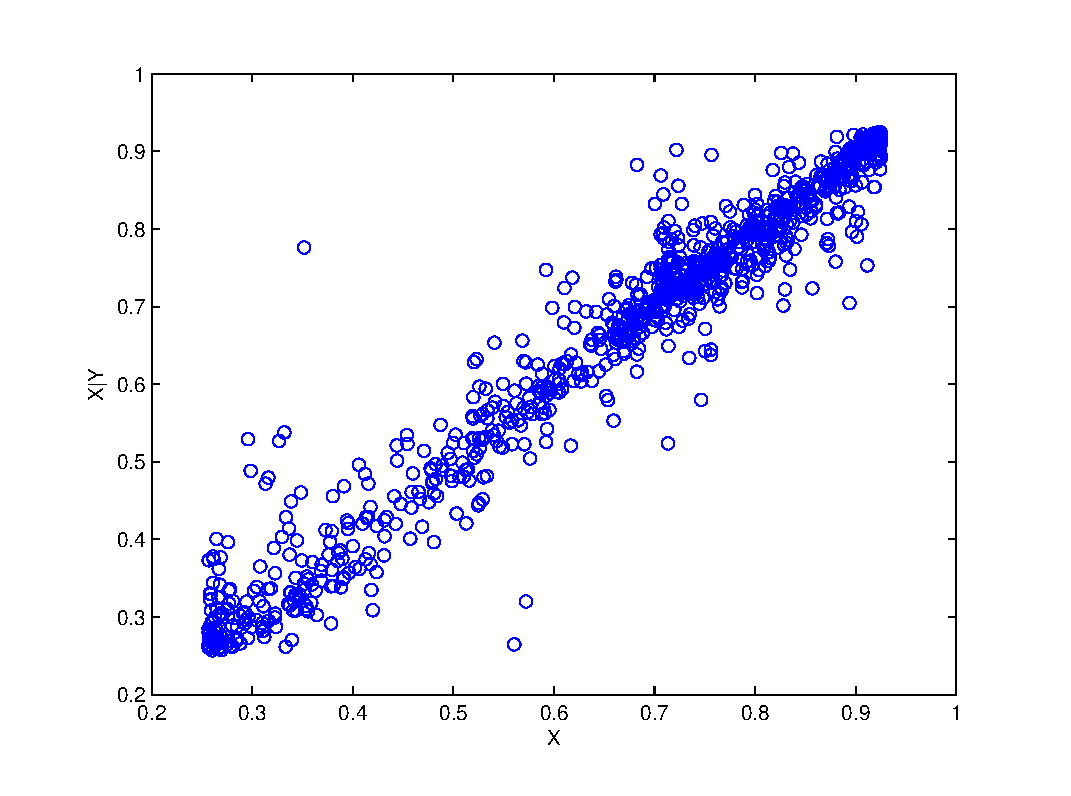
\includegraphics[scale=0.5]{RLCircuitPlots/SugFig3_XgY.eps} \\
(a) $C_{XY}$ \\[6pt]
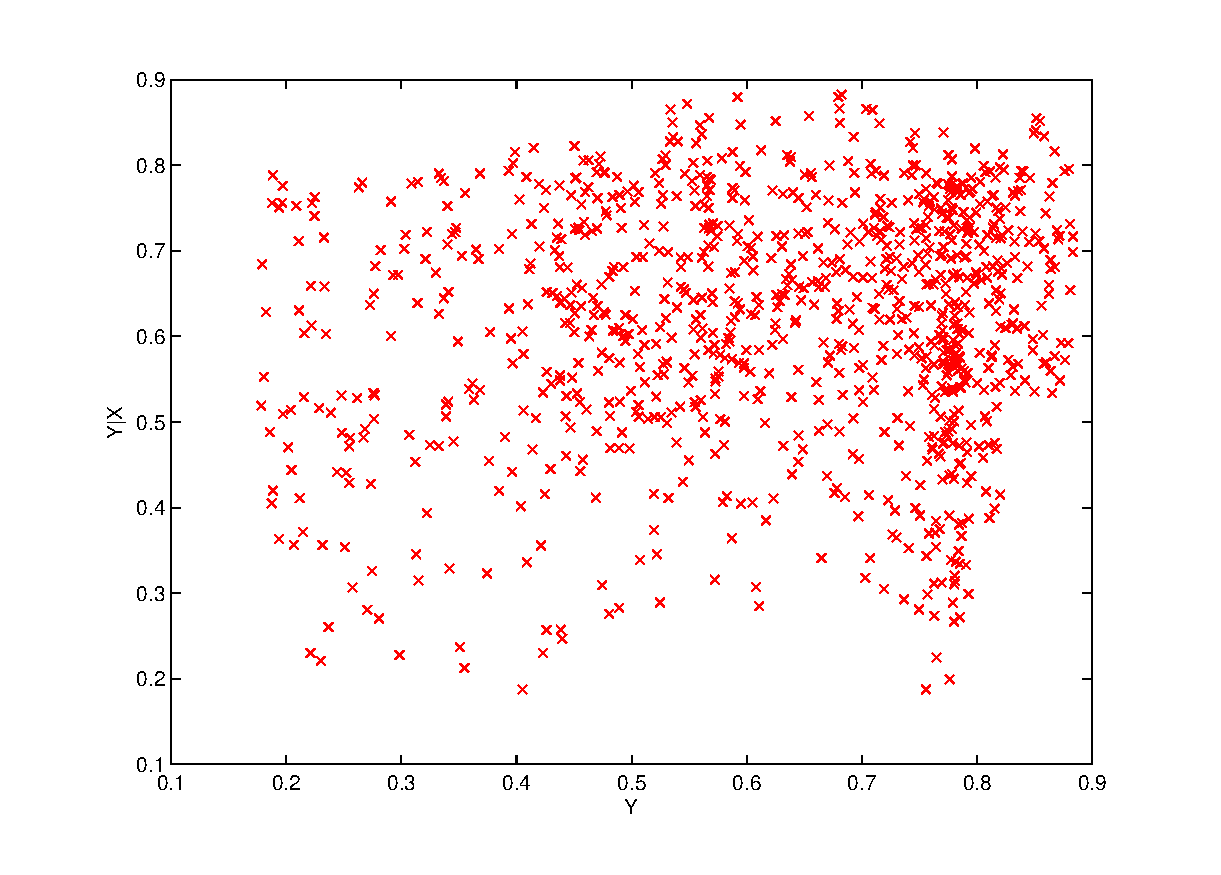
\includegraphics[scale=0.5]{RLCircuitPlots/SugFig3_YgX.eps} \\
(b) $C_{YX}$ \\[6pt]
\end{tabular}
\caption{Changing $A$ and $B$.  $C_{XY}$ and $C_{YX}$}
\label{fig1}
\end{figure}
\end{center}
This leads to

\begin{tabular}{c|c|c}
$C_{XY}$ & $C_{YX}$ & $\Delta=C_{YX}-C_{XY}$ \\
\hline \\
0.973921 & 0.110698 & -0.8632
\end{tabular}

But, these are not the only correlations that can be tested:
\begin{center}
\begin{figure}[H]
\begin{tabular}{cc}
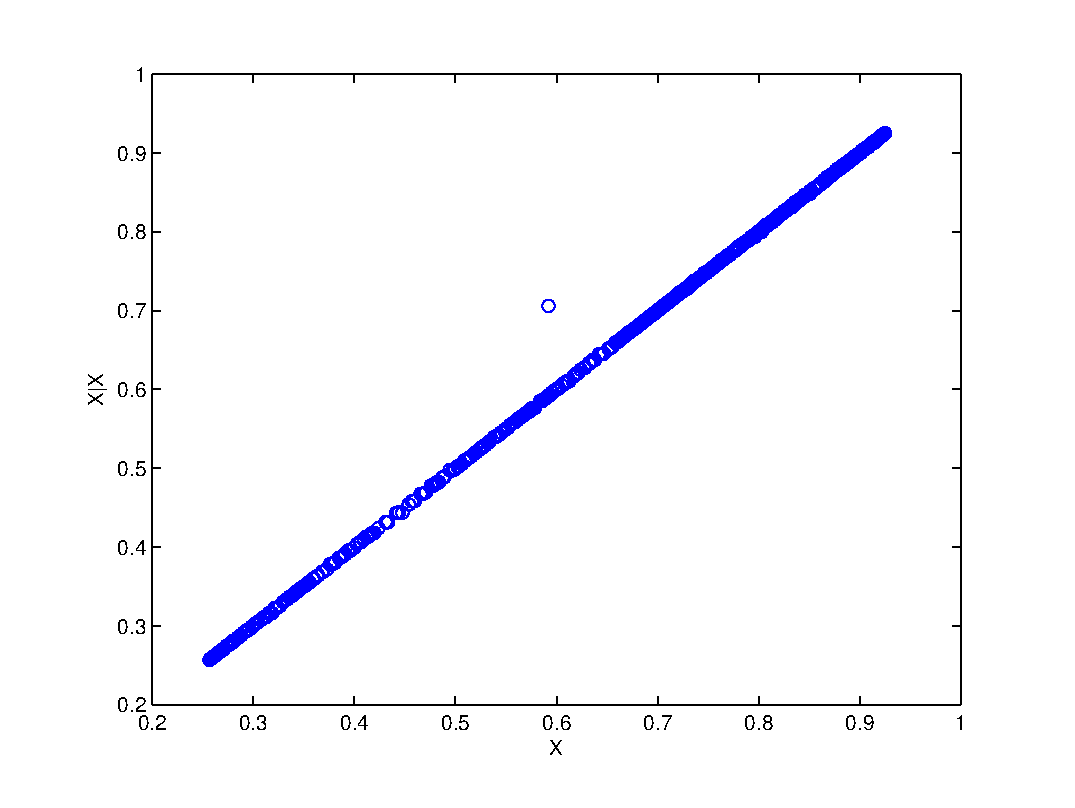
\includegraphics[scale=0.5]{RLCircuitPlots/SugFig3_XgX.eps} \\
(a) $C_{XX}$ \\[6pt]
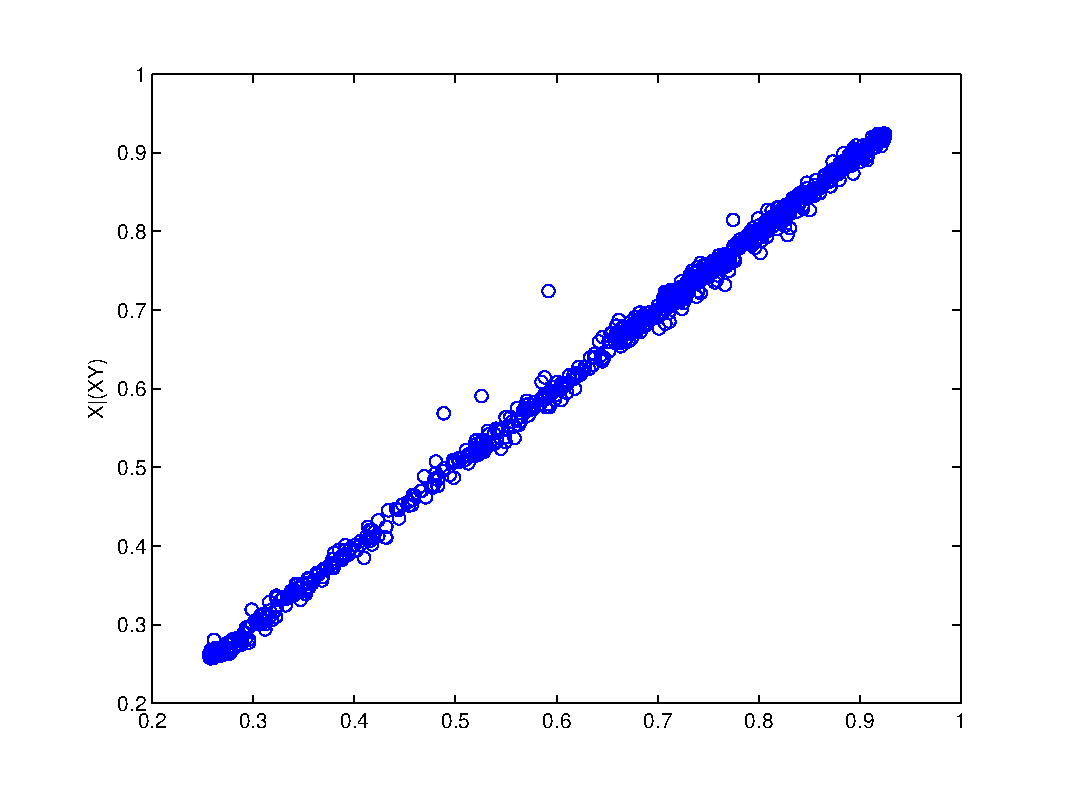
\includegraphics[scale=0.5]{RLCircuitPlots/SugFig3_XgXY.eps} \\
(b) $C_{X(XY)}$ \\[6pt]
\end{tabular}
\caption{Changing $A$ and $B$.  $C_{XY}$ and $C_{YX}$}
\label{fig1}
\end{figure}
\end{center}
\begin{center}
\begin{figure}[H]
\begin{tabular}{cc}
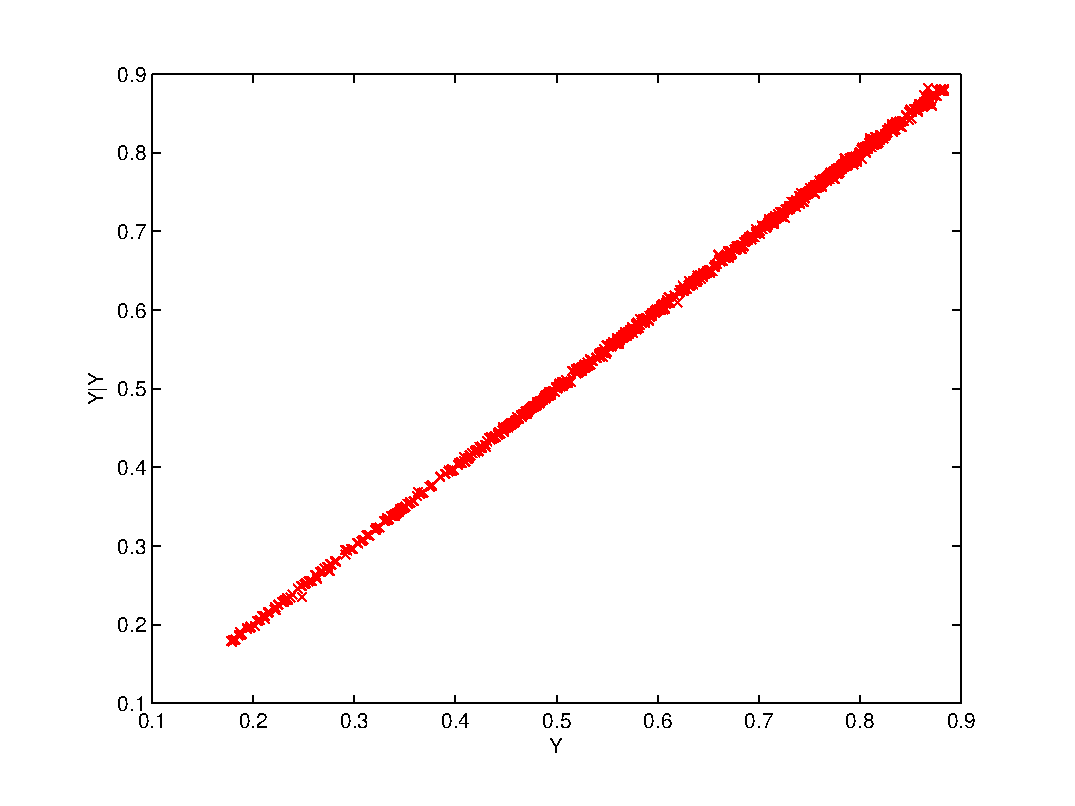
\includegraphics[scale=0.5]{RLCircuitPlots/SugFig3_YgY.eps} \\
(c) $C_{XX}$ \\[6pt]
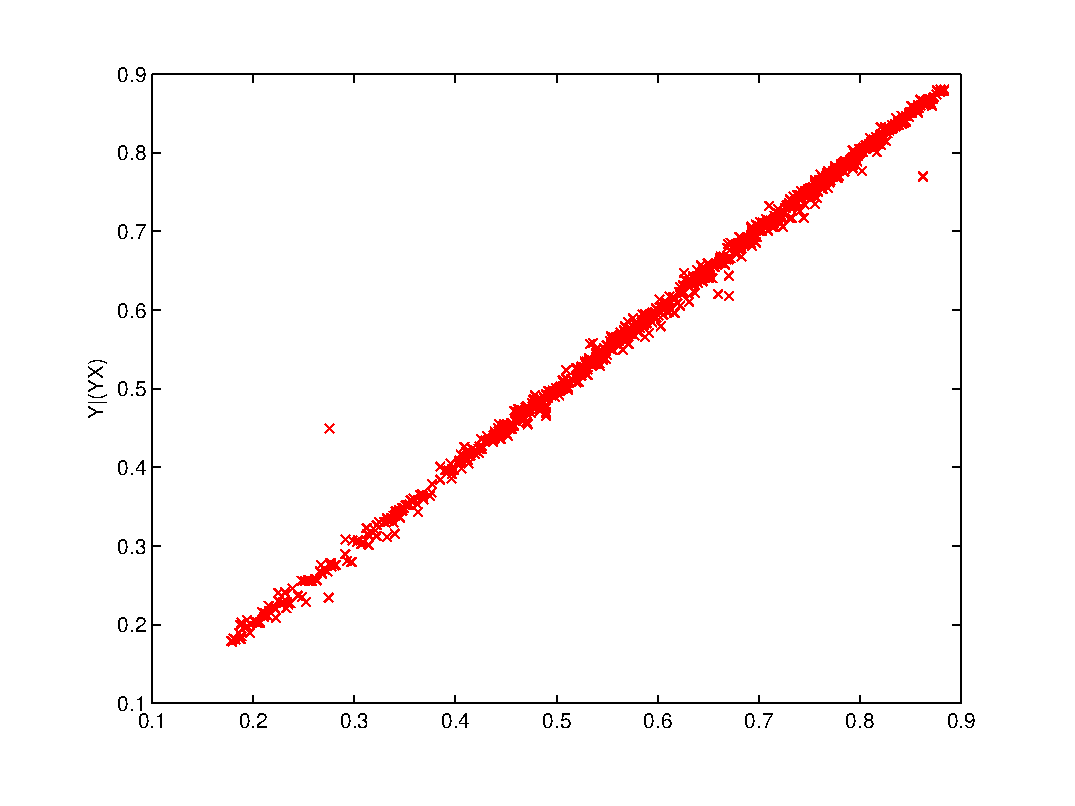
\includegraphics[scale=0.5]{RLCircuitPlots/SugFig3_YgYX.eps} \\
(d) $C_{X(XY)}$ \\[6pt]
\end{tabular}
\caption{Changing $A$ and $B$.  $C_{XY}$ and $C_{YX}$}
\label{fig1}
\end{figure}
\end{center}
This leads to

\begin{tabular}{c|c|c|c|c}
$C_{XX}$ & $C_{X(XY)}$ & $C_{YY}$ & $C_{Y(YX)}$ & $\Delta=C_{Y(YX)}-C_{X(XY)}$ \\
\hline \\
0.999841 & 0.998989 & 0.999908 & 0.998693 & -2.9548e-04
\end{tabular}

Consider a comparison of PAI and CCM given the linear example system from above.  
\begin{figure}[H]
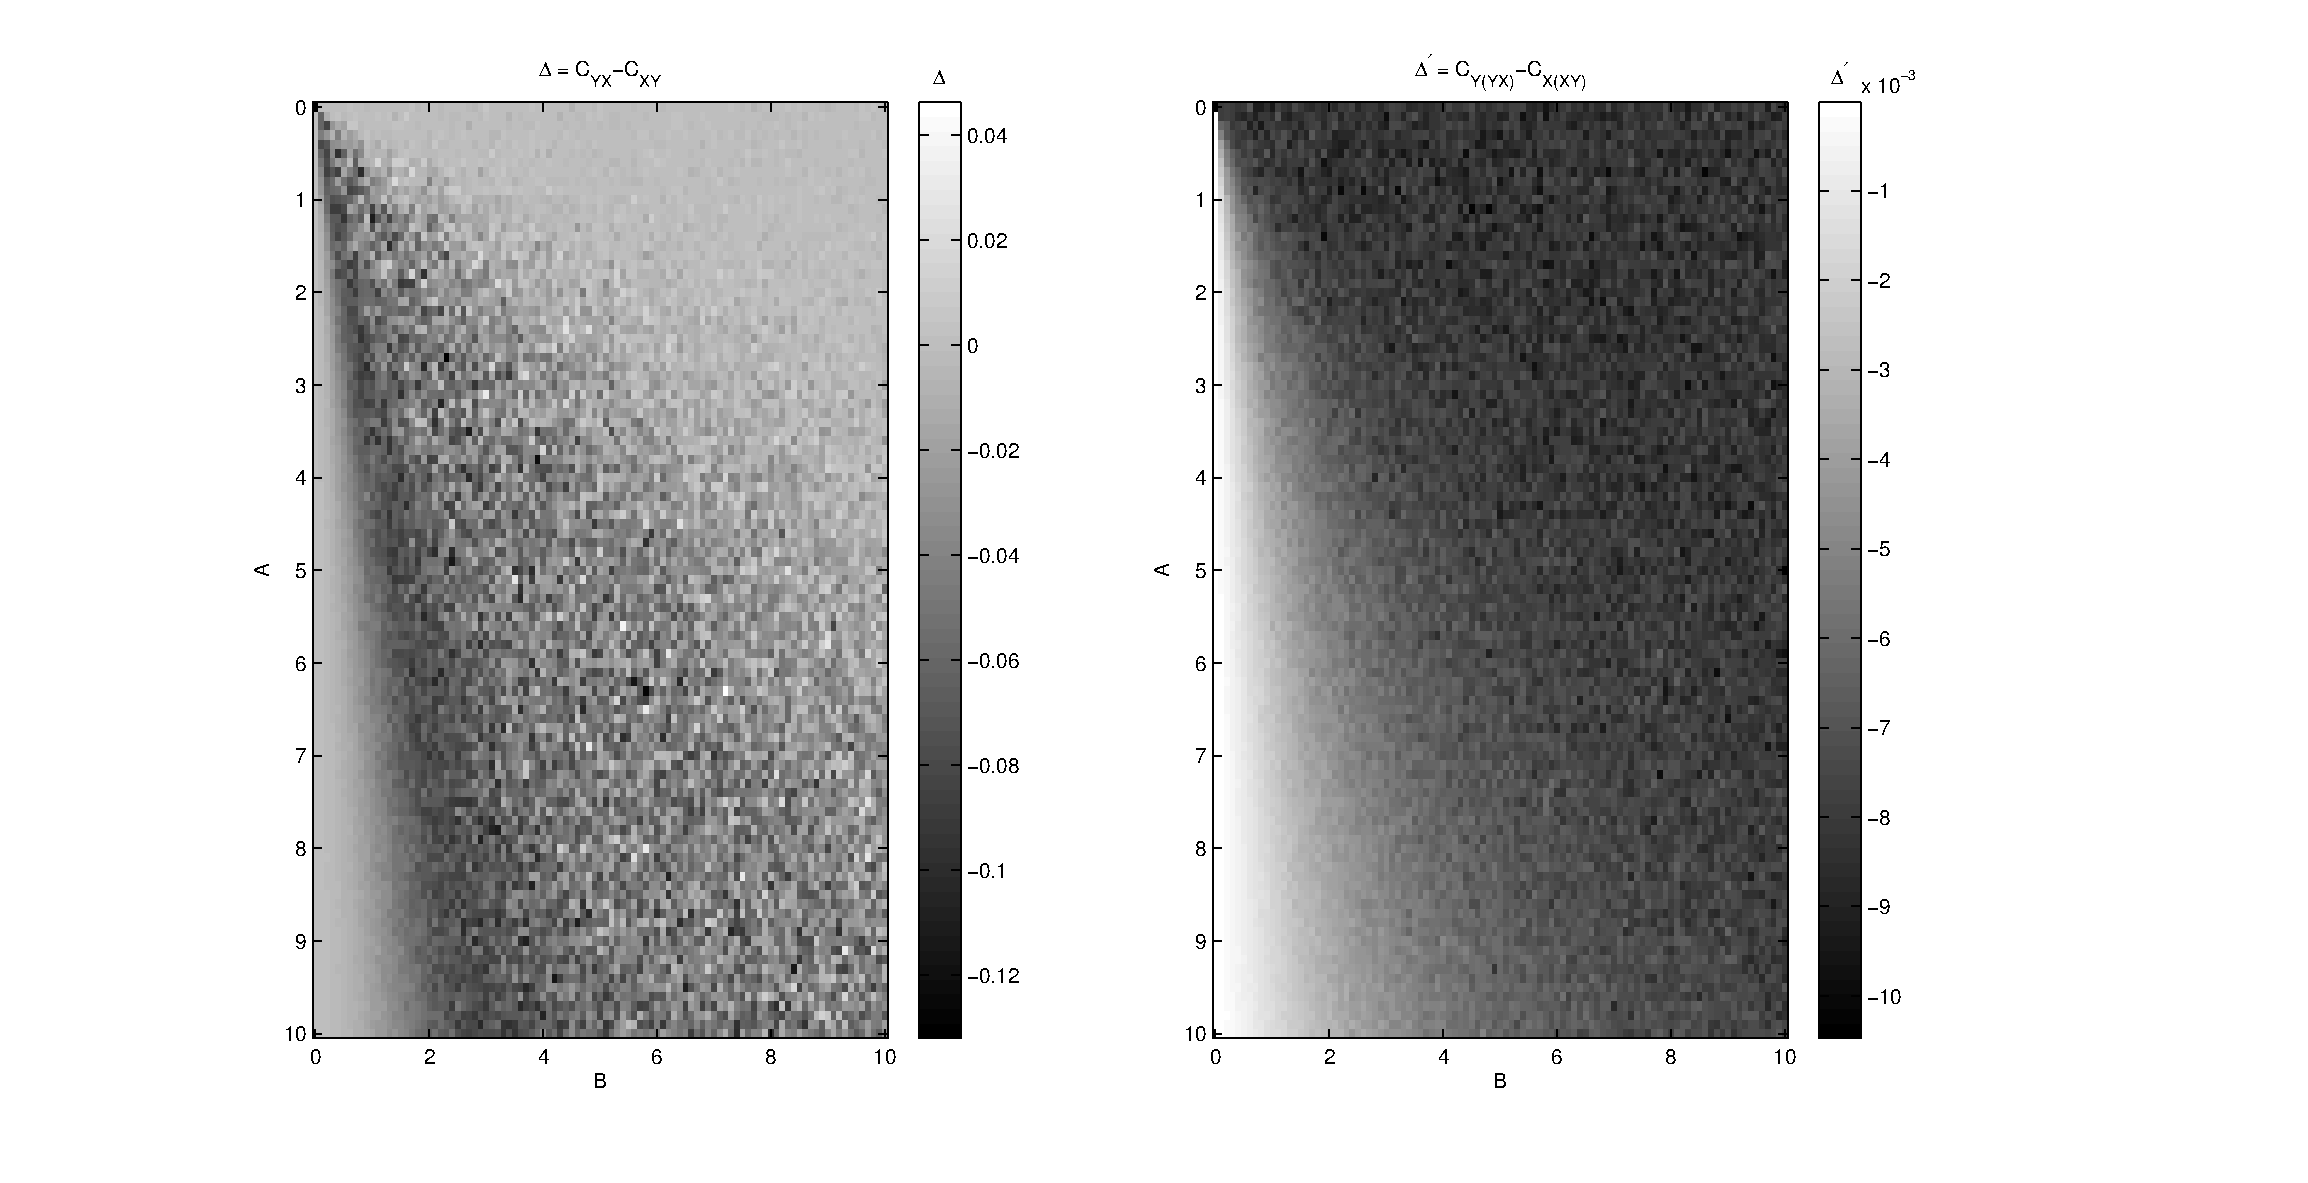
\includegraphics[scale=0.6]{RLCircuitPlots/LinearEx_PAI.eps} \\
\caption{Linear Example 1 PAI}
\label{fig1}
\end{figure}

\begin{figure}[H]
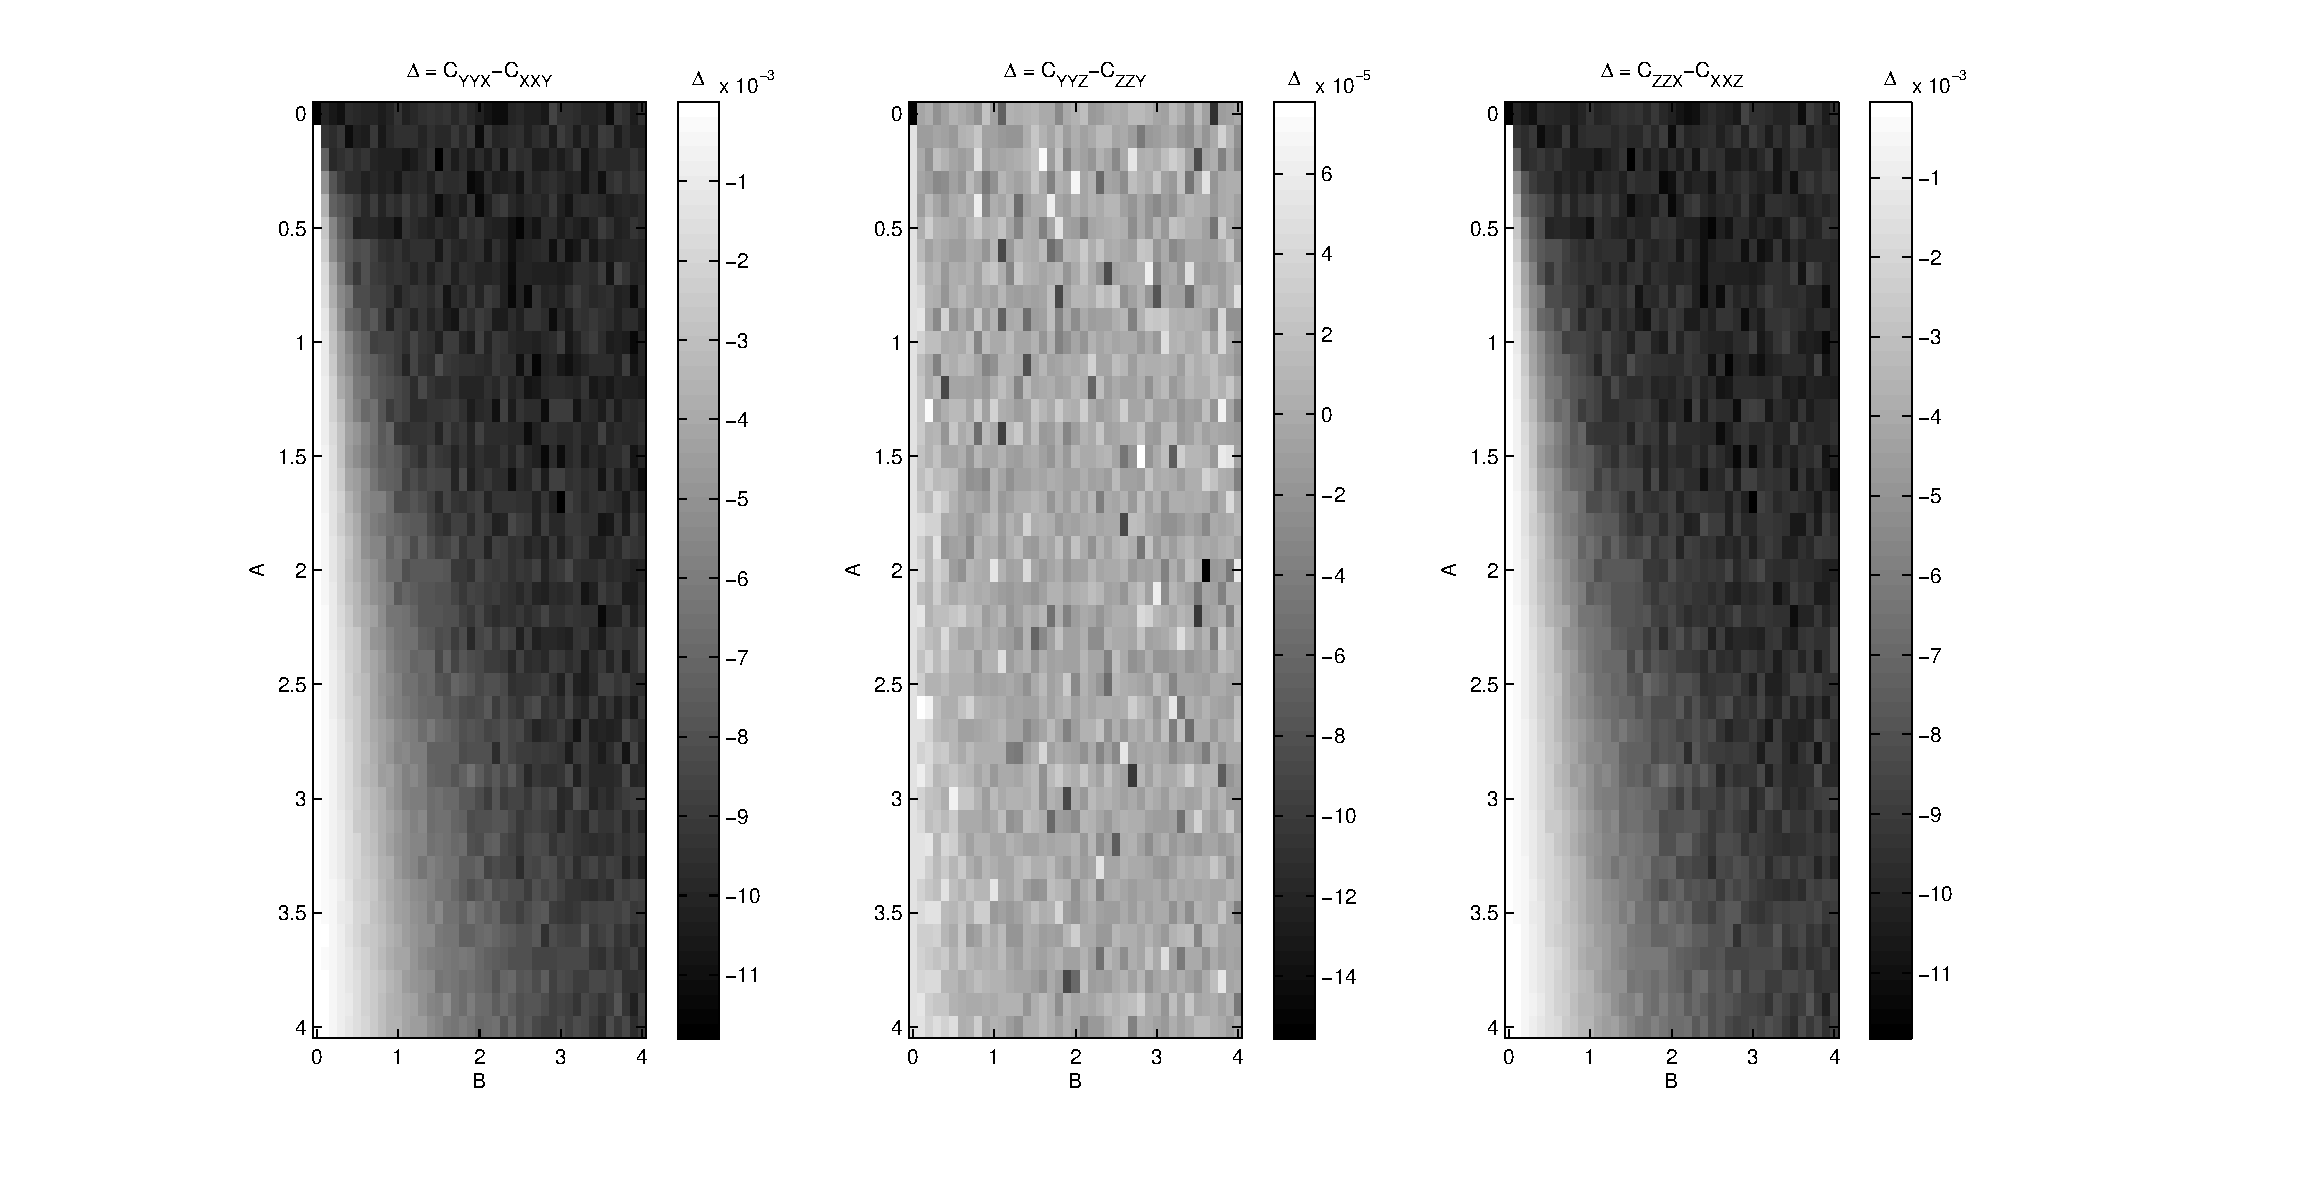
\includegraphics[scale=0.6]{RLCircuitPlots/LinearXYZPAIEx.eps} \\
\caption{Linear Example 2 PAI}
\label{fig2}
\end{figure}

\begin{figure}[H]
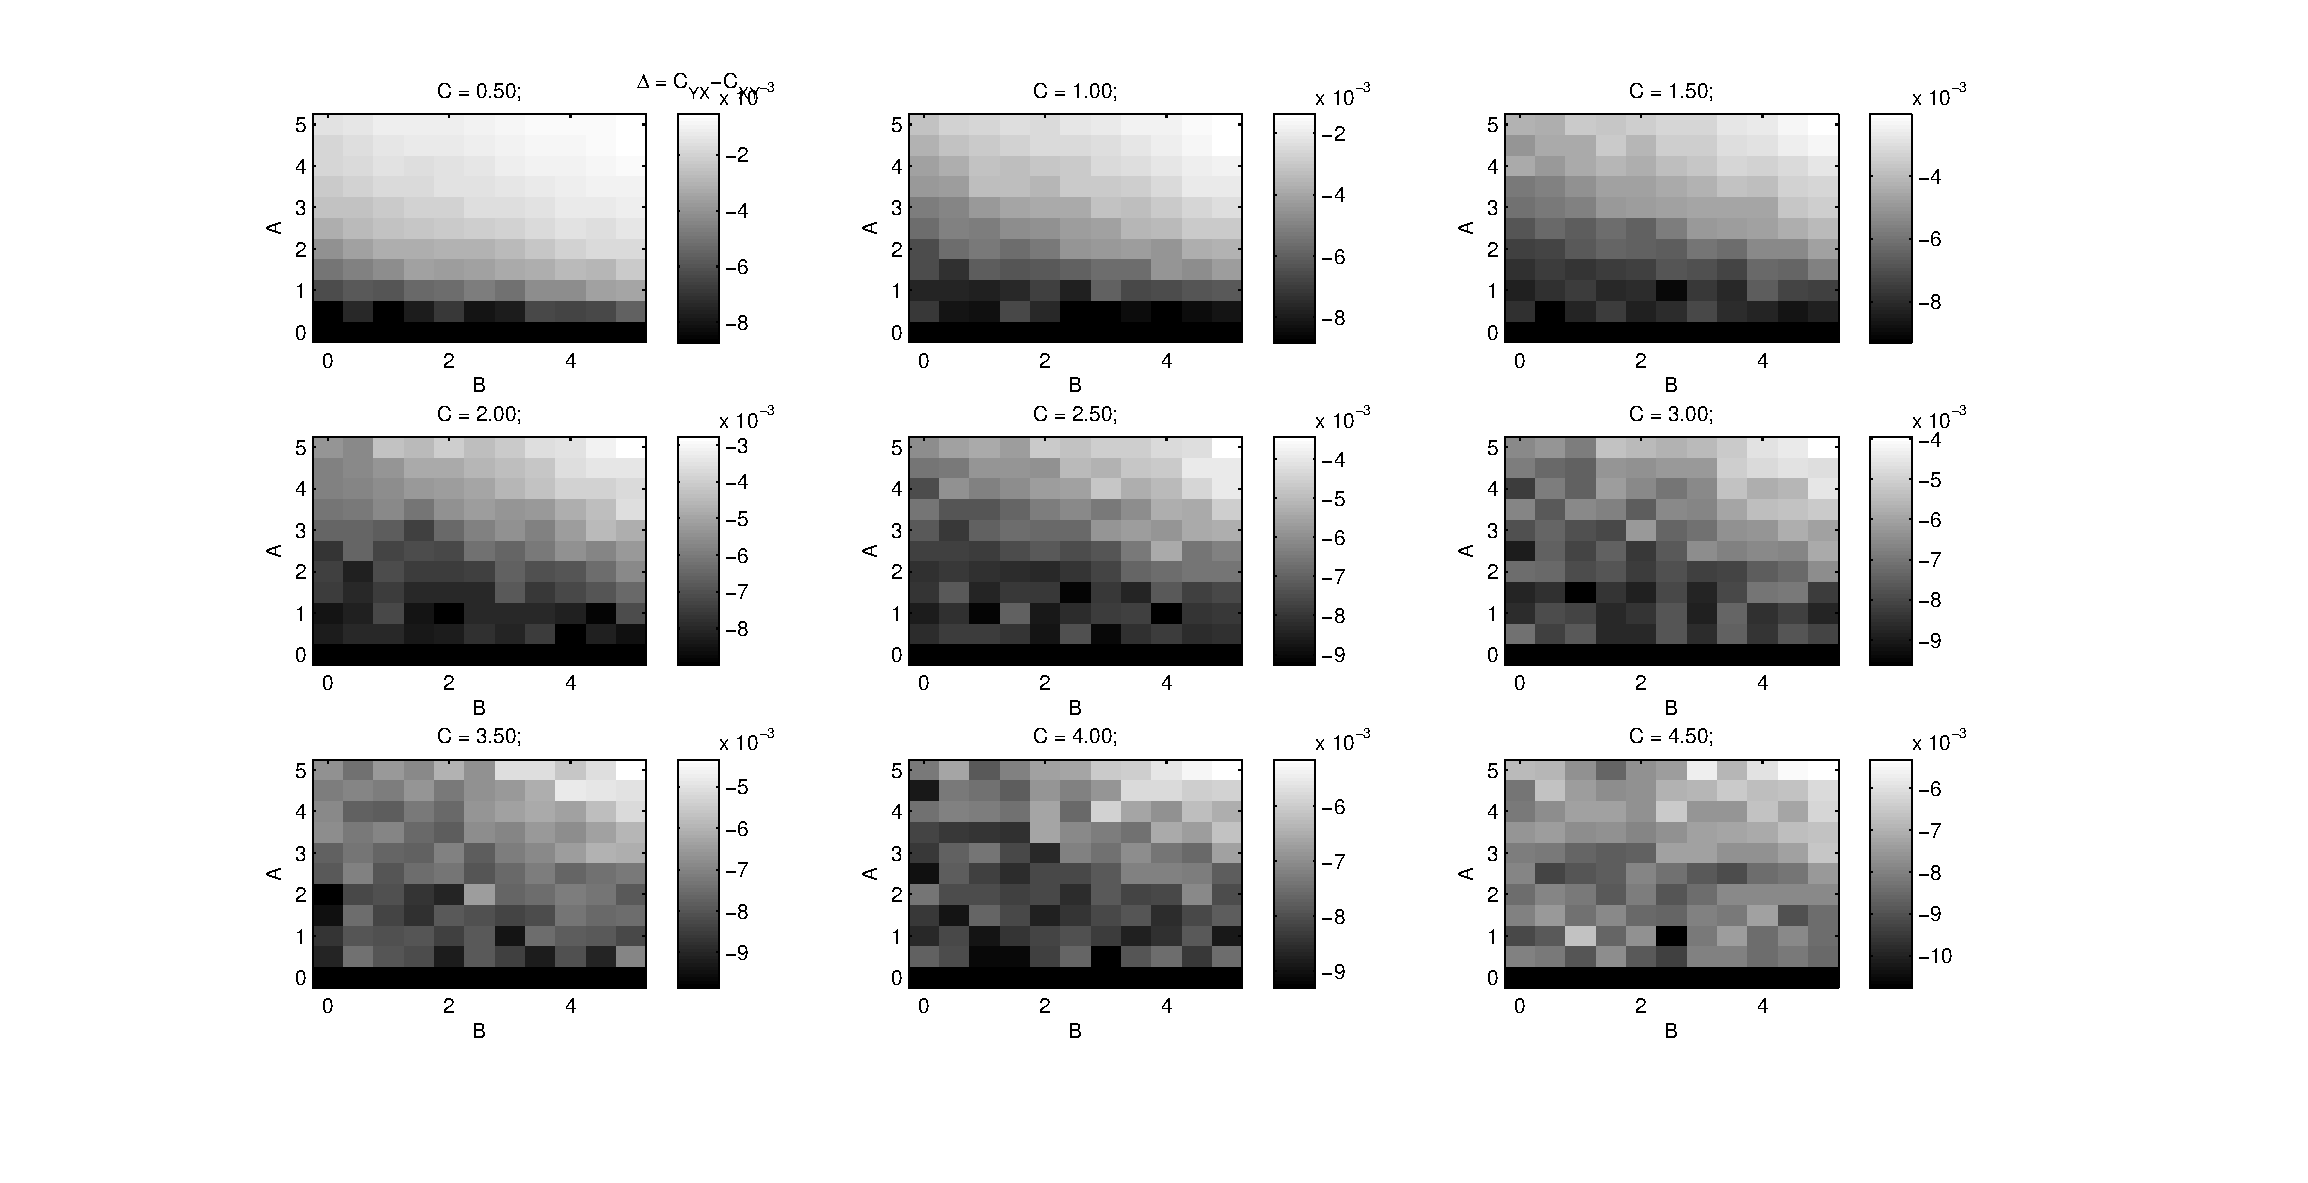
\includegraphics[scale=0.6]{RLCircuitPlots/NonLinearPAIEx.eps} \\
\caption{Non Linear Example PAI}
\label{fig2}
\end{figure}


\section{Conclusion}
{\bf Remember to state $E$ and $\tau$ for all the plots!}

A set of three time series data sets $X$, $Y$, and $Z$, would have three directed correlations (which is pairwise in the data sets by definition).  Each of the three directed correlations would determine the CCM causality as, for example, whether $X$ CCM causes $Y$, $Y$ CCM causes $X$, or ``there is no CCM causality in this system''.  The relationship stated using the phrase ``CCM causes'' indicates which time series history in the pair of data sets is the better predictor of its partner.  For example, the statement ``$X$ CCM causes $Y$'' indicates the histories (i.e.\ delay vectors) of $Y_t$ are better predictors of $X_t$ than the histories of $X_t$ are of $Y_t$.  Such information can be useful, but should not be confused with physical causality.

\section{Appendix A: CCM Algorithm}
\label{sec:appA}
A description of this algorithm is also available in \cite{Sugihara2012} (supplementary materials).  It is elucidating to partition the CCM algorithm into five distinct (though related) steps:
\begin{enumerate}
\item Create the shadow manifold for $X$, called $\tilde{X}$
\item Find the nearest neighbors to $\tilde{X}_t$
\item Use the nearest neighbors to create weights
\item Use the weights to estimate $Y$, called $Y|X$
\item Find the correlation between $Y$ and $Y|X$ 
\end{enumerate}
The steps vary in complexity and are explained in more detail below.

\subsection{Create $\tilde{X}$}
Given an embedding dimension $E$, the shadow manifold of $X$, called $\tilde{X}$, is created by associating an $E$-dimensional vector to each point $X_t$ that is constructed as $\vec{X}_t=(X_t,X_{t-\tau},X_{t-2\tau},\ldots,X_{t-(E-1)\tau}$ (this vector is often called a ``delay vector'').  The first such vector is created at $t=1+(E-1)\tau\equiv t_s$ and the last is at $t=L\equiv t_l$ where $L$ is the time series length (or ``library length'').  

\subsection{Find Nearest Neighbors}
The minimum number of points required for a bounding simplex in an $E$-dimensional space is $E+1$ (find a non-Sugihara reference for this statement).  Thus, the nearest neighbor search results is a set of distances $\{d_1,d_2,\ldots,d_{E+1}\}$ and an associated set of times $\{t_1,t_2,\ldots,t_{E+1}\}$ (where the subscript 1 denotes the closest neighbor, 2 denotes the next closest neighbor, and so on).  The distances from $\vec{X}_t$ are defined as
$$
d_i = D\left(\vec{X}_t,\vec{X}_{t_i}\right)\;\;,
$$
where $D(\vec{a},\vec{b})$ is the Euclidean distance between vectors $\vec{a}$ and $\vec{b}$.

\subsection{Create Weights}
Each nearest neighbor will be used to find an associated weight.  The unnormalized weights are defined as
$$
u_i = e^{-\frac{d_i}{d_1}}\;\;.
$$
The weights are defined as
$$
w_i = \frac{u_i}{N}\;\;,
$$
where the normalization factor is given as
$$
N = \sum_j u_j\;\;.
$$

\subsection{Find $Y|X$}
A point $Y_t$ in $Y$ can be estimated using the (normalized) distances to the points in $X$ using the weights calculated above.  This estimate is calculated as
$$
Y_t|X = \sum_i w_i Y_{t_i}\;\;.
$$

\subsection{Find the Correlation}
The CCM correlation is defined as 
$$
C_{YX} = \left(\rho\left(Y,Y|X\right)\right)^2\;\;,
$$
where $\rho_{A,B}$ is the standard Pearson's correlation coefficient between $A$ and $B$.  It can be seen from the above algorithm that $X=Y \Rightarrow C_{YX}=C_{XY}$, but in general, $C_{YX}\neq C_{XY}$.  


\bibliographystyle{plain}
\bibliography{main}

\end{document}






